\documentclass[11pt, a4paper]{article} 
\usepackage{graphicx}
\usepackage[parfill]{parskip}
\usepackage[]{natbib}
\usepackage[a4paper, margin=1in]{geometry}
\usepackage{url}
\usepackage{amsmath,amssymb,bm}
\usepackage{authblk}
\usepackage{booktabs}
\usepackage{tabularx,ragged2e}
\newcolumntype{R}[1]{>{\raggedleft\let\newline\\\arraybackslash\hspace{0pt}}m{#1}}
\newcolumntype{C}[1]{>{\centering\arraybackslash}m{#1}} 
\usepackage{caption}
\usepackage{xcolor, colortbl}
\definecolor{my-grey}{RGB}{220,220,220}
\definecolor{my-white}{RGB}{255,255,255}
\usepackage{multirow}
\usepackage{hhline}
\usepackage{lscape}
\usepackage{makecell}
\usepackage{hyperref}
\hypersetup{
	colorlinks=true,
	linkcolor=blue,
	filecolor=magenta,      
	urlcolor=black,
	citecolor=blue,
}
\setlength{\parindent}{1cm}

\begin{document}

\captionsetup[figure]{labelfont={bf},labelsep=period}
\captionsetup[table]{labelfont={bf},labelsep=period}

\title{A Three-component Approach to Model and Forecast\\ Age-at-death Distributions}	
\author[1,2]{Ugofilippo Basellini\thanks{Corresponding author: \url{ugofilippo.basellini@ined.fr}}}
\author[1]{Carlo Giovanni Camarda}
\affil[1]{\small \textit{Institut national d'\'{e}tudes d\'emographiques (INED), Paris}}
\affil[2]{\small \textit{Interdisciplinary Centre on Population Dynamics (CPOP), Department of Public Health, University of Southern Denmark, Odense}}

\maketitle
\thispagestyle{empty}

\begin{abstract}

Mortality forecasting has recently received growing interest, as accurate projections of future lifespans are needed to ensure the solvency of insurance and pension providers. Several innovative stochastic methodologies have been proposed in most recent decades, the majority of them being based on age-specific mortality rates or on summary measures of the life table. The age-at-death distribution is an informative life-table function that provides readily available information on the mortality pattern of a population, yet it has been mostly overlooked for mortality projections. In this chapter, we propose to analyse and forecast mortality developments over age and time by introducing a novel methodology based on age-at-death distributions. Our approach starts from a nonparametric decomposition of the mortality pattern into three independent components corresponding to Childhood, Early-adulthood and Senescence, respectively. We then model the evolution of each component-specific death density with a relational model that associates a time-invariant standard to a series of observed distributions by means of a transformation of the age axis. Our approach allows us to capture mortality developments over age and time, and forecasts can be derived from parameters' extrapolation using standard time series models. We illustrate our methods by estimating and forecasting the mortality pattern of females and males in two high-longevity countries using data of the Human Mortality Database. We compare the forecast accuracy of our model and its projections until 2050 with three other forecasting methodologies. 

\end{abstract}	

\bigskip

\noindent \textbf{Keywords:} Mortality forecasting$\;\cdot\;$Mortality modelling$\;\cdot\;$Relational models$\;\cdot\;$Smoothing$\;\cdot\;$\\Mortality decomposition$\;\cdot\;$Life expectancy$\;\cdot\;$Lifespan variability

\section{Introduction}\label{Sec:Intro}

Population projections and mortality forecasts have been studied since the beginning of the twentieth century. The seminal works of \cite{whelpton1928population,whelpton1936empirical} and \cite{lotka1939theorie} on the cohort component method and the stable population contributed significantly to the development and application of population projections. Mortality forecasts go back at least to the beginning of the twentieth century, as actuaries were concerned about the financial effects of mortality improvements on life annuities and pensions \citep{pollard1987projection}. It is however in the last three decades that mortality forecasting flourished, owing to the introduction and development of stochastic methodologies to project mortality. 

Three functions can be used to analyse human mortality and its developments over age and time: the hazard, the survival and the probability density function \citep{klein2005survival}. These functions describe the same stochastic phenomenon and are uniquely related between each other: one can derive any two of them by knowing the third one, without the need of additional information. 

Despite the complementarity of the mortality functions, the majority of forecasting techniques is based on age-specific mortality rates or death probabilities \citep[for comprehensive reviews, see][]{booth2008mortality,cairns2009quantitative,shang2011point,stoeldraijer2013impact}. Most of these models take advantage of the regularities typically found in age- and time-patterns, such as the predominantly downward trend in age-specific mortality observed in many developed countries during the last 60 years, and they extrapolate the trends in the future using statistical methods \citep{haberman2011comparative}. 

Nevertheless, the inspection of the other two functions can provide additional insights on mortality developments that one might not directly discern from a rate-based analysis. It is well known that the remarkable mortality improvements observed in these countries during the twentieth century are generally divided into two stages of mortality changes: compression and shifting dynamics \cite[see, for example,][]{fries1980aging,wilmoth1999rectangularization,kannisto2000measuring,bongaarts2005long,canudas2008modal}. Broadly speaking, the first stage took place in the first part of the century, as significant reductions in infant and childhood mortality resulted in grater equality in lengths of life. In the second part of the century, mortality improvements at older ages became more prominent, resulting in higher average lifespans with stagnating equality. 

The age-at-death distribution is an excellent function to inspect these dynamics of mortality changes. Mortality compression can be detected from the reduction in the variability of the distribution, while shifting corresponds to a translation of the distribution to higher ages without relevant changes in its shape. In addition, the distribution provides immediate information on key questions in mortality studies, such as the longevity of the population, and the inequality in ages at death.

Figure \ref{Fig:Intro} shows changes in the age-at-death distribution of Swiss males between 1950 and 2016. The graphical inspection of the death distribution readily provides information on the population's longevity, which is typically measured by life expectancy at birth or, in low mortality countries, by the modal age at death \citep{kannisto2001mode,horiuchi2013modal}. Additionally, the variability of lifespans within the population can be directly assessed from the spread of the distribution or its interquartile range. The increase in longevity as well as the reduction of lifespan variability for Swiss males during this period clearly emerge from Figure \ref{Fig:Intro}. Moreover, changes in the distribution over time highlight the two dynamics of mortality: for example, it is evident that the shifting dynamic of mortality started around the 1970-1980s, becoming more prominent in most recent decades, while the compression dynamic had been strongest in the decades {\color{red}1950-1970 and 1990-2010}.
  
\begin{figure}[t]
	\begin{center}
		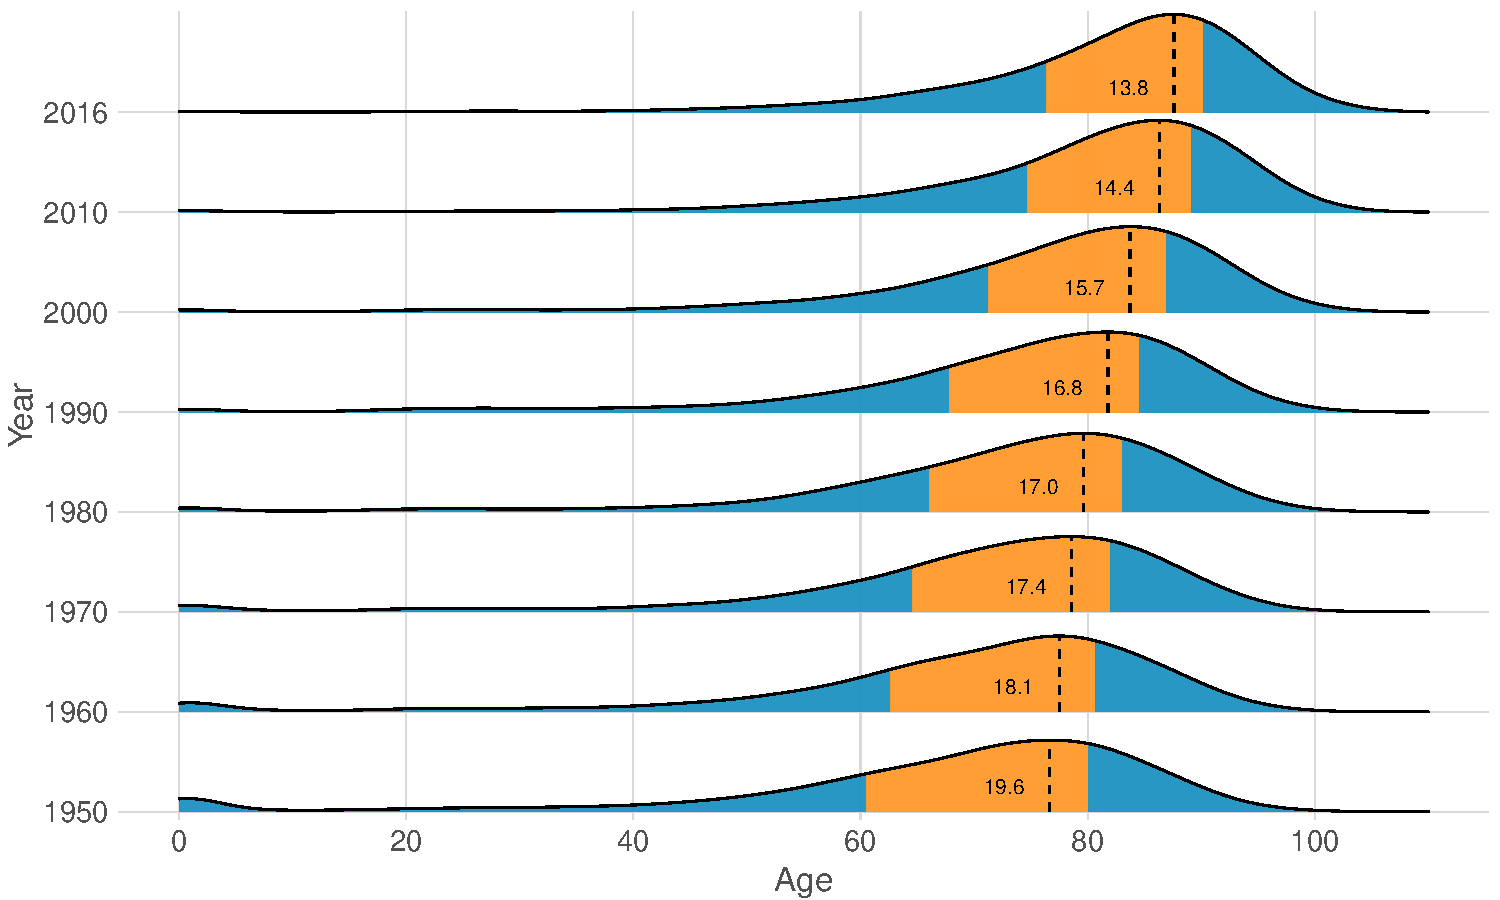
\includegraphics[scale=0.55]{./Figures/F1.pdf}
		\caption{Changes in the age-at-death distribution for Swiss males at selected years between 1950 and 2016. The orange area corresponds to the interquartile range of the distribution, whose value is reported in print. The dashed line depicts the modal age at death. Data have been smoothed for illustrative purposes.\\\footnotesize{\textit{Source}: authors' own elaborations on data retrieved from the \cite{HMD}.} \label{Fig:Intro}}		
	\end{center}
\end{figure}

Despite providing direct information on mortality patterns and trends over time, surprisingly few methods have been proposed to forecast mortality from age-at-death distributions. Among the firsts to abandon the conventional approach of using mortality rates, \cite{oeppen2008coherent} and \cite{oeppen2013coherent} proposed to forecast the density of single and multiple-decrement life tables, using methodologies borrowed from compositional data analysis. \cite{bergeron2017coherent} expanded on this work, suggesting a coherent model based on life-table deaths of fifteen Western European countries. Furthermore, \cite{basellini2019stad} proposed a relational model to forecast adult mortality from age-at-death distributions. Finally, \cite{pascariu2019maximum} suggested a vector autoregressive model to forecast the statistical moments of the death distribution.
  
In this chapter, we contribute to the growing literature of forecasting the age-pattern of mortality from age-at-death distributions. Specifically, we extend the Segmented Transformation Age-at-death Distributions (STAD) model proposed by \cite{basellini2019stad}, which focuses on adult mortality only, to obtain mortality forecasts for the entire age range. While retaining the underlying methodology of the STAD model, here we introduce significant novelties to achieve our goal. In particular, our approach is based on two steps. First, we decompose the observed death counts into three additive mortality components, namely Childhood, Early-adulthood and Senescent mortality. We perform this decomposition via the nonparametric approach proposed by \cite{camarda2016sums}. Secondly, we model and forecast each component-specific age-at-death distribution employing specialized versions of the STAD model. As such, the Three-Component STAD (3C-STAD) model allows us to capture mortality developments over the entire age range, and forecasts are obtained from the extrapolation of the model's parameters using standard time-series techniques. 

This chapter is organized as follows. In Section \ref{Sec:Methods}, we overview the methods that we introduce as well as the data that we employ. In Section \ref{Sec:Results}, we provide two illustrations of our methodology by forecasting female and male mortality in two high-longevity countries. In particular, we first assess the accuracy of point and interval forecasts of the 3C-STAD model by performing three out-of-sample validation exercises. We then present the 3C-STAD forecasts until the year 2050. In both cases, we compare the 3C-STAD with three other well-known forecasting methodologies. Finally, in Section \ref{Sec:Discussion} we summarize and discuss our results. 

\section{Methods}\label{Sec:Methods}

\subsection{Mortality functions}\label{Subsec:MortFun}

Human mortality can be analysed by any one of three complementary functions: the hazard, the survival and the probability density function \citep{klein2005survival}. In demography, for a given calendar year $t$, these functions are generally known as the force of mortality $\mu(x,t)$ at age $x$, the probability of surviving from birth to age $x$, $\ell(x,t)$, and the age-at-death distribution $f(x,t)$. 

The three mortality functions are uniquely related between each other, and knowing one of them allows to determine the other two. In the following, without loss of generality, let $\ell(0, t)$, commonly labelled as the life-table radix, be equal to one, and let us drop the time index $t$ to ease notation. The relationship that exists between the three functions at any age $x$ is given by:
%
\begin{equation}\label{Eq:DxfromLxMx}
f(x)  = \ell(x)\,\mu(x)\,.
\end{equation}
%
The probability of surviving  $\ell(x)$ can be derived from the other two mortality functions:
%
\begin{equation}\label{Eq:LxfromMx}
\ell(x) = \mathrm{exp} \left(- \int_{0}^{x} \mu (a)da\right)\,, \quad \ell(x) = \int_{x}^{\omega} f(x)\,dx\,,
\end{equation}
%
where $\omega$ is the highest age attained in the population. Thus, combining \eqref{Eq:DxfromLxMx} and \eqref{Eq:LxfromMx} demonstrates the complementarity of the three mortality functions.

Since \cite{thiele1871mathematical}, demographers and actuaries described human mortality into three different components that operates principally, or almost exclusively, upon childhood, middle and old ages, respectively. The attempt to decompose those three components stimulated numerous approaches (cf.~Section \ref{Sec:Discussion}). In a general setting, the hypothesis can be expressed as follows:
%
\begin{equation}\label{Eq:MxDecomp}
	\mu(x)=\mu_{c}(x)+\mu_{e}(x)+\mu_{s}(x)  \, ,
\end{equation}
%
where the force of mortality $\mu(x)$ at age $x$ is additively decomposed into three independent components, $\mu_{c}(x)$, $\mu_{e}(x)$, and $\mu_s(x)$. For ease of presentation, we labelled these mortality component with Childhood, Early-adulthood and Senescence, respectively. However, they theoretically operate over all ages $x$. Combining \eqref{Eq:DxfromLxMx} and \eqref{Eq:MxDecomp}, the corresponding decomposition of the age-at-death distribution can be written as follows: 
%
\begin{align}\label{Eq:FxDecom}
f(x) & = \ell(x)\,\mu_{c}(x) + \ell(x)\,\mu_{e}(x) + \ell(x)\,\mu_{s}(x) \notag \\
& = f_{c}(x)+f_{e}(x)+f_{s}(x) \, . 
\end{align}
%

\subsection{Data and mortality decomposition}\label{Subsec:DataMortDecomp}
Whereas risk of death acts continuously, mortality functions and models can be displayed only at particular ages and years. For modelling and forecasting mortality and for a specific sex and population, available data are thus observed death counts, $d_{x,t}$, and central exposures to the risk of death, $e_{x,t}$, with ages $x=0,\dots,\omega$ and years $t$. In the following, we analyse the female and male populations of two high-longevity countries, Sweden and Switzerland, choosing a common time period (1950-2016) and with $\omega=110+$. While Sweden was selected for the high standard in data quality, even at the oldest ages \citep{vaupel1994longer,wilmoth1996extreme}, Switzerland was chosen for its atypical mortality development, especially for males, related to the strong HIV epidemic during the 1980s \citep{csete2012switzerland}. Data are taken from the \citeauthor{HMD} (HMD, \citeyear{HMD}). 

We assume that the number of deaths at age $x$ and year $t$ is a random variable $D_{x,t}$ that follows a Poisson process \citep{brillinger1986biometrics}:
\begin{equation}\label{Eq:Poisson}
D_{x,t} \sim \mathcal{P}(e_{x,t} \; \mu_{x,t}) 
\end{equation}
where the force of mortality $\mu_{x,t}$ is assumed to be constant over each year of age (i.e.~from age $x$ to $x+1$) and over each calendar year (i.e.~from year $t$ to $t+1$). This assumption implies that $\mu_{x,t}$ approximates the force of mortality at exact age $x+\frac{1}{2}$ and exact time $t+\frac{1}{2}$ \citep{cairns2009quantitative}. Note that the notation $\mu_{x,t}$ is the discrete counterpart of the continuous notation $\mu(x,t)$ employed in Subsection \ref{Subsec:MortFun}. Moreover, death rates $m_{x,t} = d_{x,t}/e_{x,t}$ are the maximum likelihood estimators of the force of mortality $\mu_{x,t}$, if no structure is enforced over age and/or time. 
 
The first step in the Three-Component Segmented Transformation Age-at-death Distributions (3C-STAD) model concerns the decomposition of the force of mortality into its three independent components $\mu_k(x)$, $k=c,e,s$. Instead of employing a parametric mortality model, we favour a non-parametric approach to avoid imposing a rigid structure and achieve a better fit to the observed data. For this purpose, we employ the Sum of Smooth Exponentials (SSE) model, which has been shown to provide insightful results for mortality analysis \citep{camarda2016sums,remund2018young}. In the following, we provide a short overview of the SSE model; for a more detailed description of the model, we refer the interested reader to the original paper of \cite{camarda2016sums}.

The SSE belongs to the class of multiple-component models \cite[also known as competing hazard models,][]{gage1993decline}, as it proposes an additive decomposition of the expected value of counts in multiple (smooth) components. In a given year $t$, let $\bm{\mu}$, $\bm{d}$ and $\bm{e}$ denote vectors over age of overall force of mortality, death counts and exposures, respectively. Within the SSE, we can model the force of mortality as the sum of three components $\bm{\gamma}=\left[\bm{\gamma}_c:\bm{\gamma}_e:\bm{\gamma}_s\right]'$. The expected value of the Poisson process $\bm{d} \sim \mathcal{P}(\bm{e}\,\bm{\mu})$ is expressed as a composition of exposures and mortality components, i.e.~$\bm{e}\,\bm{\mu} = \bm{C}\,\bm{\gamma}$, where the composition matrix $\bm{C}=\left[\bm{E}:\bm{E}:\bm{E}\right]$ is a block matrix that includes three times the diagonal matrix of population exposures $\bm{E}=\mathrm{diag}(\bm{e})$ (one for each component of mortality). The composition matrix has the dual role of multiplying each component by the exposure times and of summing them to obtain the overall Poisson mean. The SSE model can be framed as a Composite Link Model \citep{thompson1981composite}, and estimation of the model's parameters can be obtained by a modified version of the iterative reweighted least squares (IWLS) algorithm \citep{eilers2007ill}.  

The SSE model has several advantages over parametric decompositions of the force of mortality, which made it our favoured choice for the first step of the 3C-STAD. Although the SSE could accommodate parametric assumptions, it allows to model each component by assuming only smoothness over age (and eventually over time). We opted for this last more flexible setting. This can be achieved by expressing each component $k$ as a linear combination of $B$-spline basis $\bm{B}_k$ and associated coefficients $\bm{\alpha}_k$: 
\begin{equation}\label{Eq:SSEcomponent}
\bm{\gamma}_k = \mathrm{exp} \left( \bm{B}_k\,\bm{\alpha}_k\right), \quad k=c,e,s. 
\end{equation}
Smoothness of $\bm{\gamma}_k$ is obtained by combining a large number of $B$-splines and a roughness penalty on the coefficients vector $\bm{\alpha}_k$ \citep{eilers1996flexible}. Note that the exponential in \eqref{Eq:SSEcomponent} guarantees positive component-specific force of mortality, as one would expect. Furthermore, component-specific shape constraints can be easily specified and included in the estimation procedure by additional asymmetric penalties. Here, we enforce monotonic decreasing and increasing constraints on the Childhood and Senescent components, respectively, and a log-concave shape for the Early-adulthood component. These constraints further aid the identifiability of the model by ensuring that the three components are not interchangeable.

Another advantage of the SSE methodology is that it adequately blends the transitions between components, without imposing sharp delimitations where one stops and another one continues. Moreover, we employ the two-dimensional extension of the SSE model. In this way we both account for the significant age-time interactions and avoid abrupt changes over time in the interaction of the components. A detailed description of year-to-year mortality fluctuations is relevant in a forecasting perspective. In the SSE model, at the cost of overfitting, this flexibility is achieved by a large number of $B$-splines with a low smoothing parameter in the time dimension.

Figure \ref{Fig:SSEexample} shows an example of fitting the two-dimensional SSE model to Swiss males between 1950 and 2016: the three components of mortality clearly emerge, each one featuring the expected shape. Unlike the original SSE model, we start our analysis from age 0 which is treated in a specific manner. This particular age represents a clear discontinuity in the age-pattern of mortality, as mortality of newborns is sharply higher than death rates at later infant ages due to malformations, pre-term births and birth-related complications \citep{chiang1984life,camarda2016sums}. Hence, we incorporate the discontinuity in the first age of life by including, for the Childhood component, a specialized coefficient for this age, which is not penalized over age. 

\begin{figure}[t]
	\begin{center}
		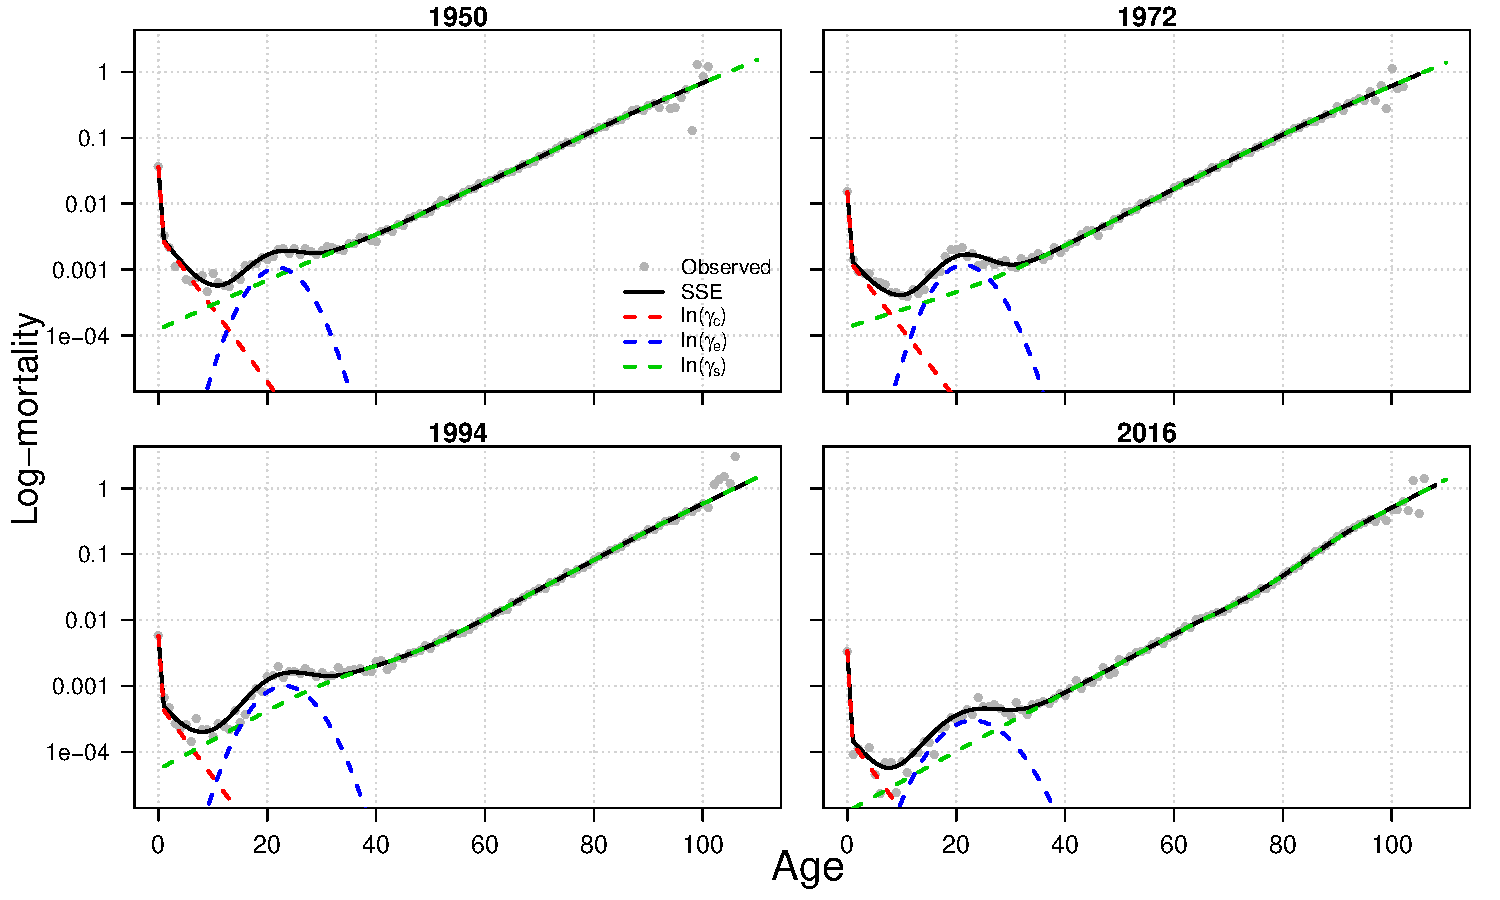
\includegraphics[scale=0.62]{./Figures/F2.pdf}
		\caption{Observed and fitted mortality rates (in log scale) for Swiss males at selected years between 1950 and 2016. The force of mortality is decomposed into Childhood ($\bm{\gamma}_c$), Early-adulthood ($\bm{\gamma}_e$) and Senescent ($\bm{\gamma}_s$) components via the two-dimensional SSE model.\\\footnotesize{\textit{Source}: as for Figure \ref{Fig:Intro}.} \label{Fig:SSEexample}}		
	\end{center}
\end{figure}

Outcomes from the SSE model allow us to obtain (i) the age-at-death distribution of each component over time {\color{red} \cite[using standard life-table construction,][]{preston2001demogr}}, and (ii) the expected number of deaths separated by component, $\hat{\bm{d}}_k=\bm{e}\,\hat{\bm{\gamma}}_k$. This allows us to model and forecast age-at-death distributions independently for each component. 

%%%%%%%%%%%%%%%%%%%%%%%%%%%%%%%%%%----------------------------%%%%%%%%%%%%%%%%%%%%%%%%%%%%%%%%%%----------------------------

\subsection{Modelling component-specific distributions}\label{Subsec:STADbyComp}

The second step of the 3C-STAD consists in modelling the component-specific age-at-death distributions. Since different features characterize the three components, we deal differently with each one of them. 

\subsubsection{Senescent mortality}
We start by presenting the model employed for the Senescent component, originally proposed and described in greater details in \cite{basellini2019stad}.
The Segmented Transformation Age-at-death Distributions (STAD) is a relational model that relates a fixed time-invariant reference distribution, denoted standard, to a series of observed distributions via a segmented transformation of the age axis. In general, consider two age-at-death distributions $f(x)$ and $g(x)$, where the former is the standard, and the latter any observed distribution. The STAD model can be expressed as $g(x) = f\left[t(x;\bm{\theta})\right]$, where the transformation function $t(x;\bm{\theta})$ is characterized by three parameters $\bm{\theta}$ that depend on: (i) the difference in modal ages at death between the two distributions, and (ii) the change in the variability of the two distributions  \textit{before} and \textit{after} their modal ages. 

Let $\nu_{s} = M_{s}^{g} - M_{s}^{f}$ denotes the difference between the mode of the Senescent distributions $g_{s}(x)$ and $f_{s}(x)$. The transformation function of the STAD model for the Senescent component, $t_{s}(\cdot)$, can then be written as: 
%
\begin{equation}\label{Eq:STADsen}
	t_{s}(x;\;\nu_{s},b_{s}^{\ell},b_{s}^{u}) = \left\{ \begin{array}{ll}
		M_{s}^{f} + b_{s}^{\ell} \, \tilde{x} \quad & \mathrm{if} \; x \leq M_{s}^{g} \\
		M_{s}^{f} + b_{s}^{u} \, \tilde{x} \quad & \mathrm{if} \; x >  M_{s}^{g} \\
	\end{array}
	\right.
\end{equation}
%
where $\tilde{x} = x - \nu_{s} - M_{s}^{f}$, and $b_{s}^{\ell}$ and $b_{s}^{u}$ denote the change in the variability of $g_{s}(x)$ with respect to $f_{s}(x)$ before and after the mode, respectively. Note that the superscript $\ell$ and $u$ refer to the lower and upper segments of the age range (i.e.~before and after the modal age at death). 

\begin{figure}[h!]
	\begin{center}
		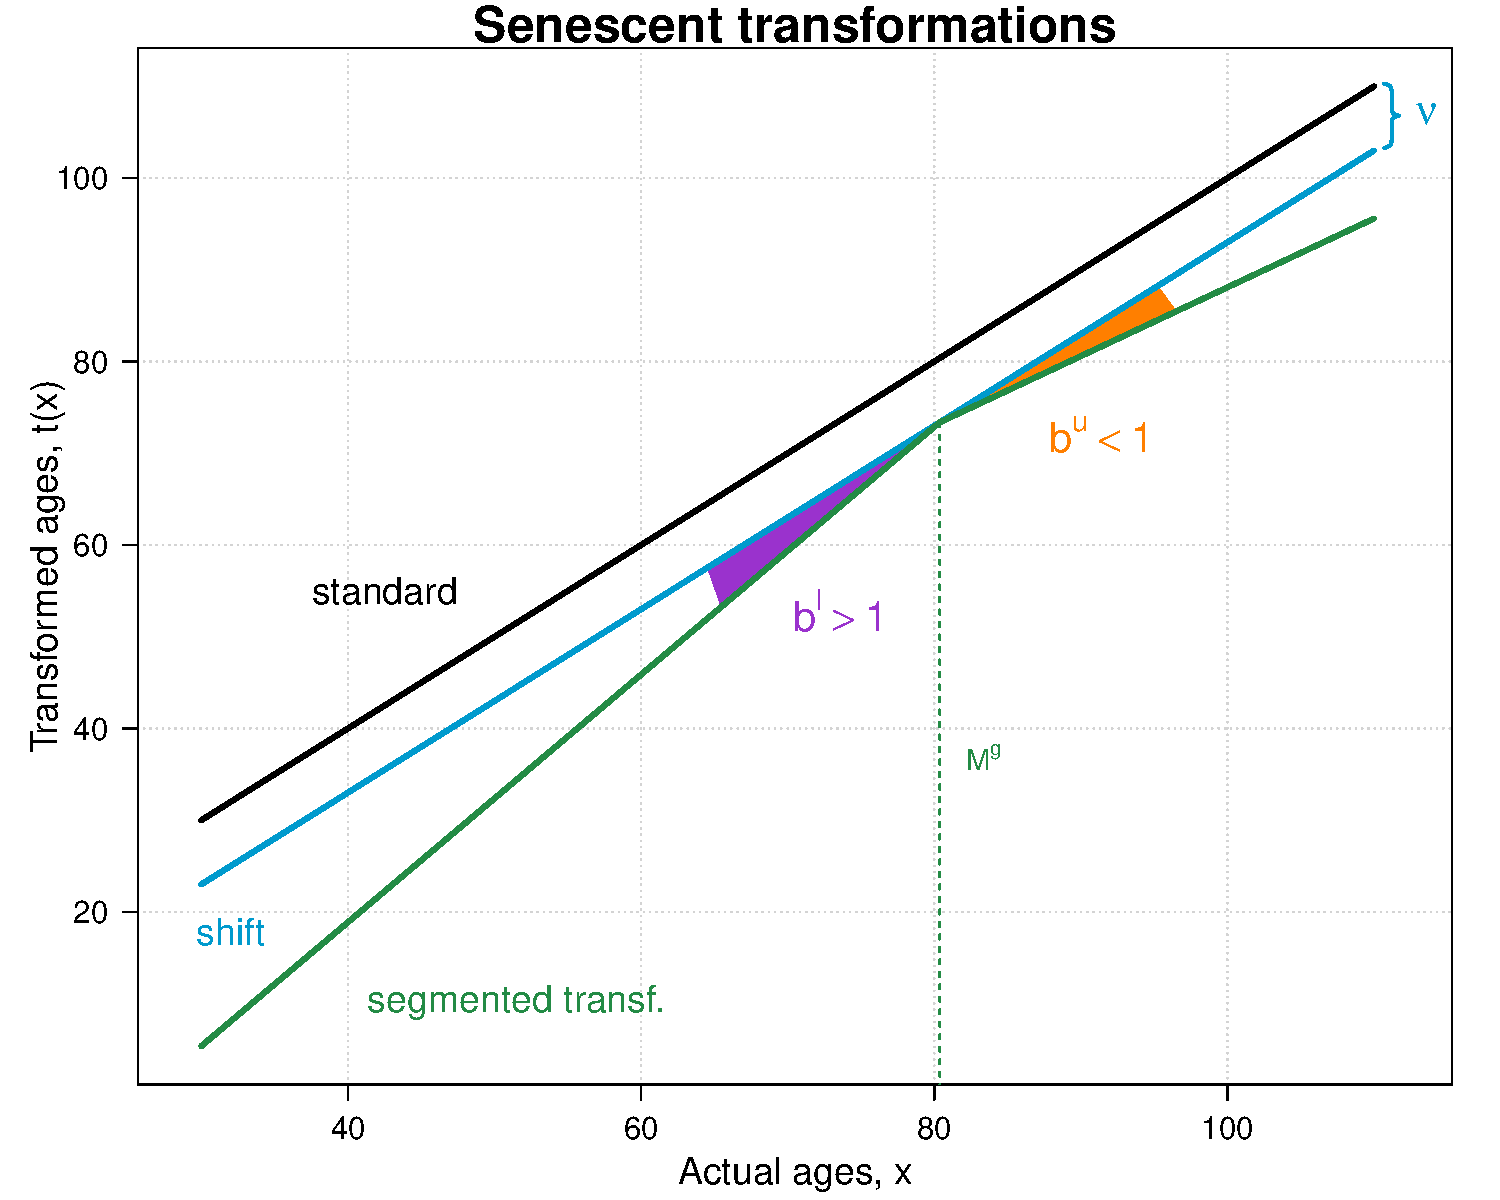
\includegraphics[scale=0.32]{./Figures/F3a.pdf}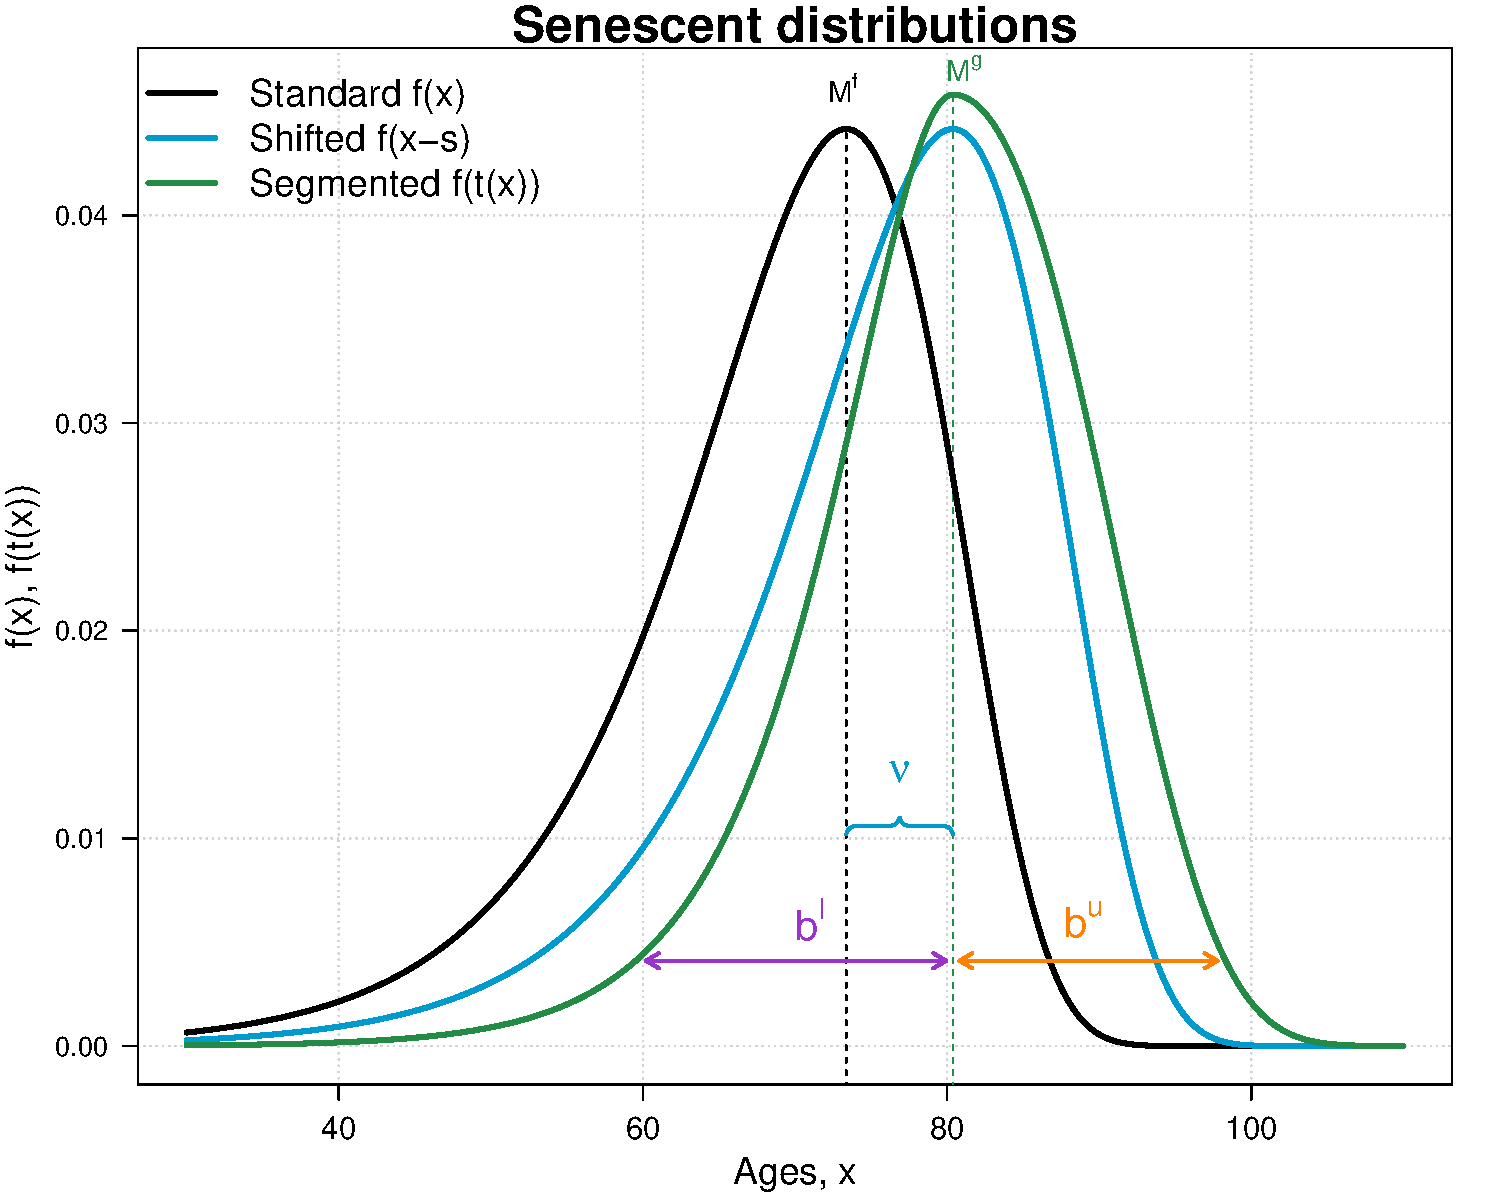
\includegraphics[scale=0.32]{./Figures/F3b.pdf}
		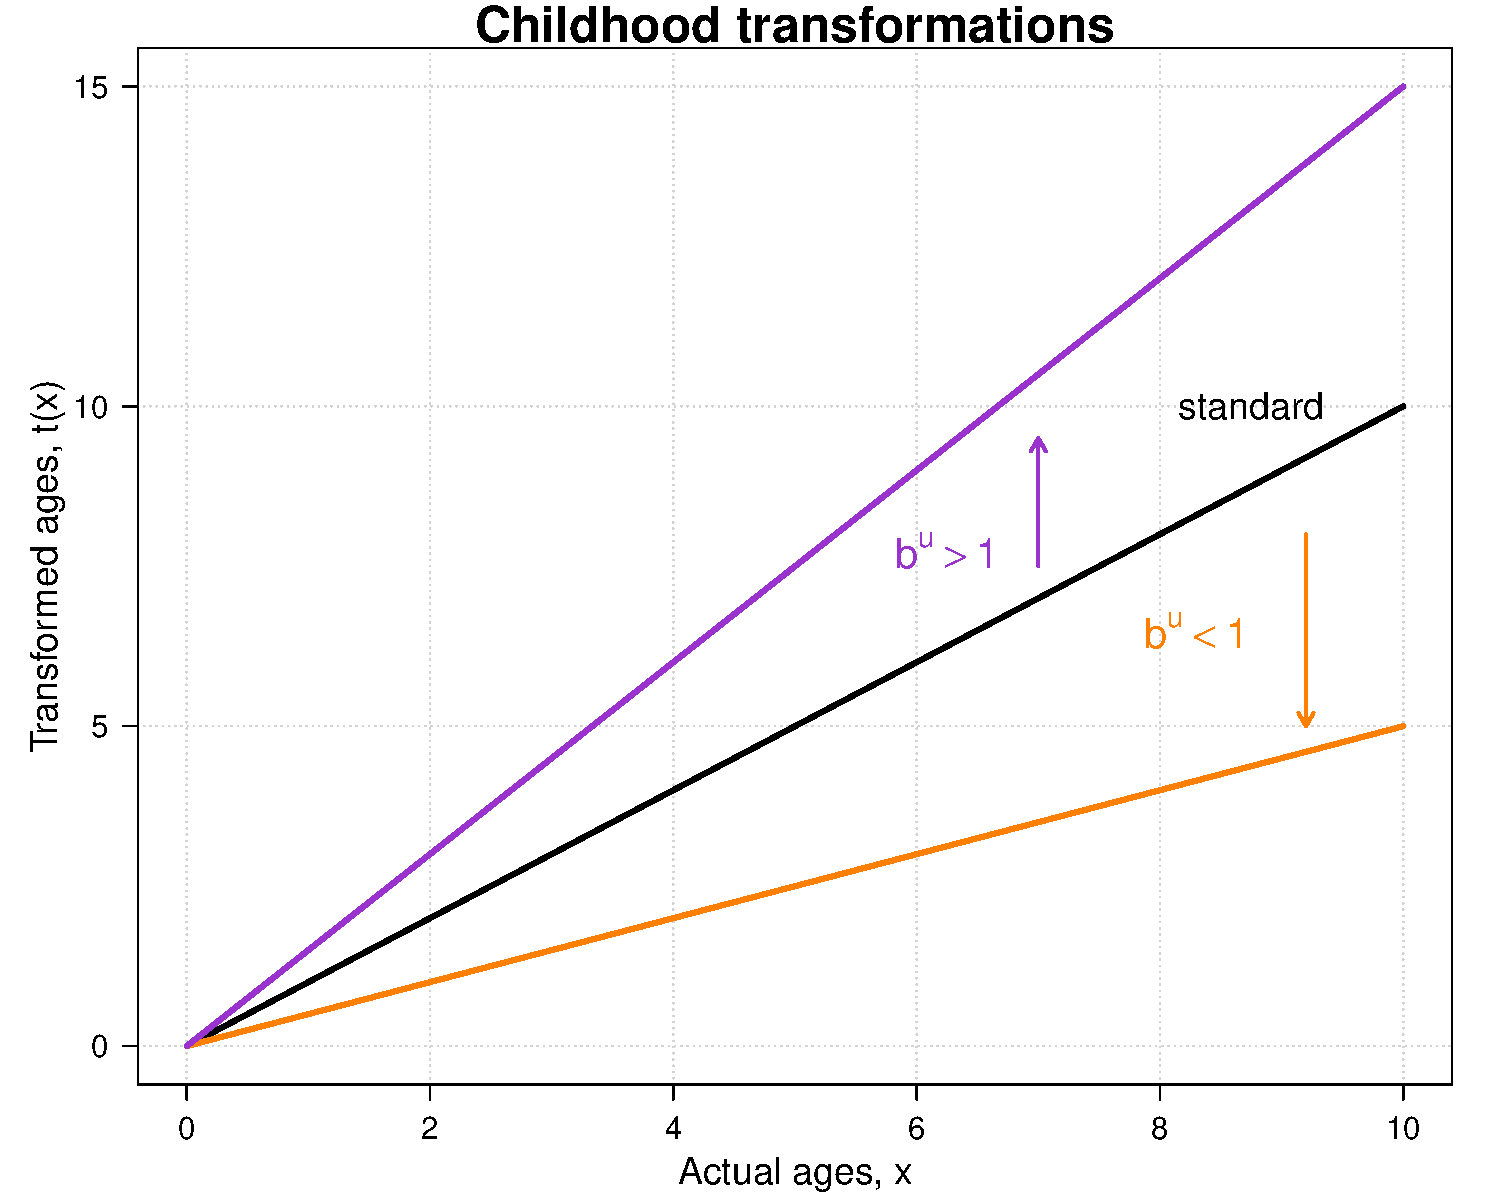
\includegraphics[scale=0.32]{./Figures/F3c.pdf}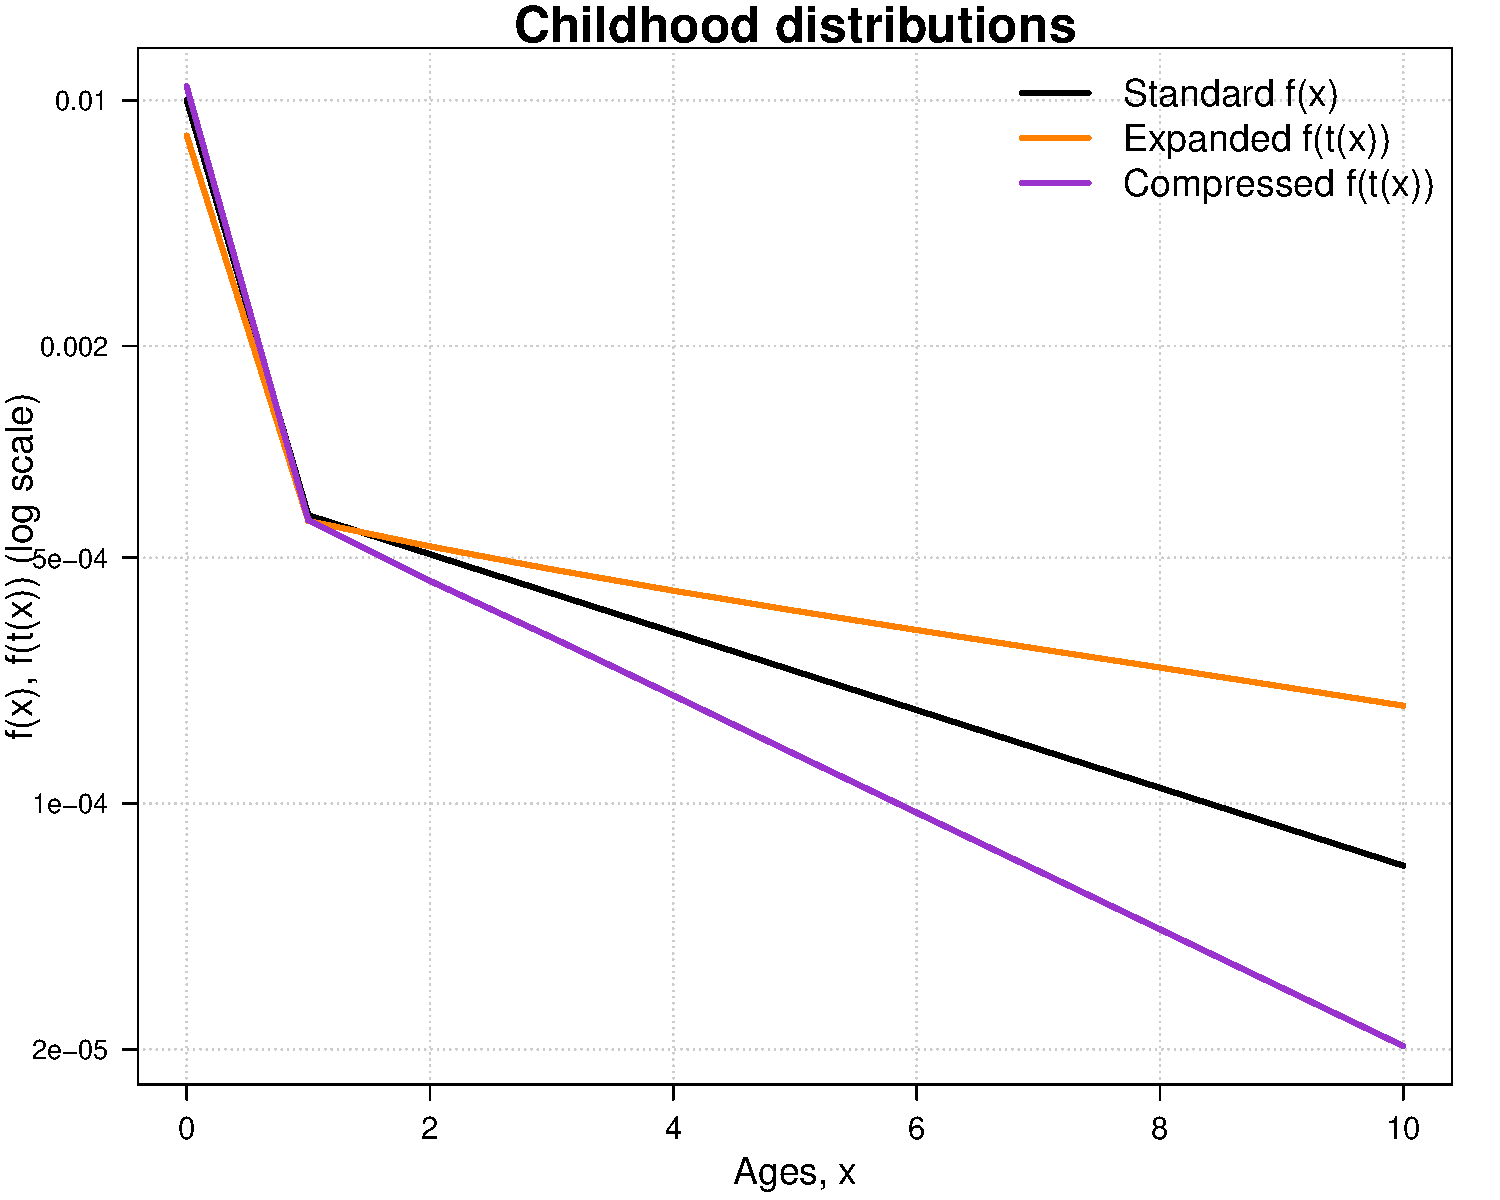
\includegraphics[scale=0.32]{./Figures/F3d.pdf}
		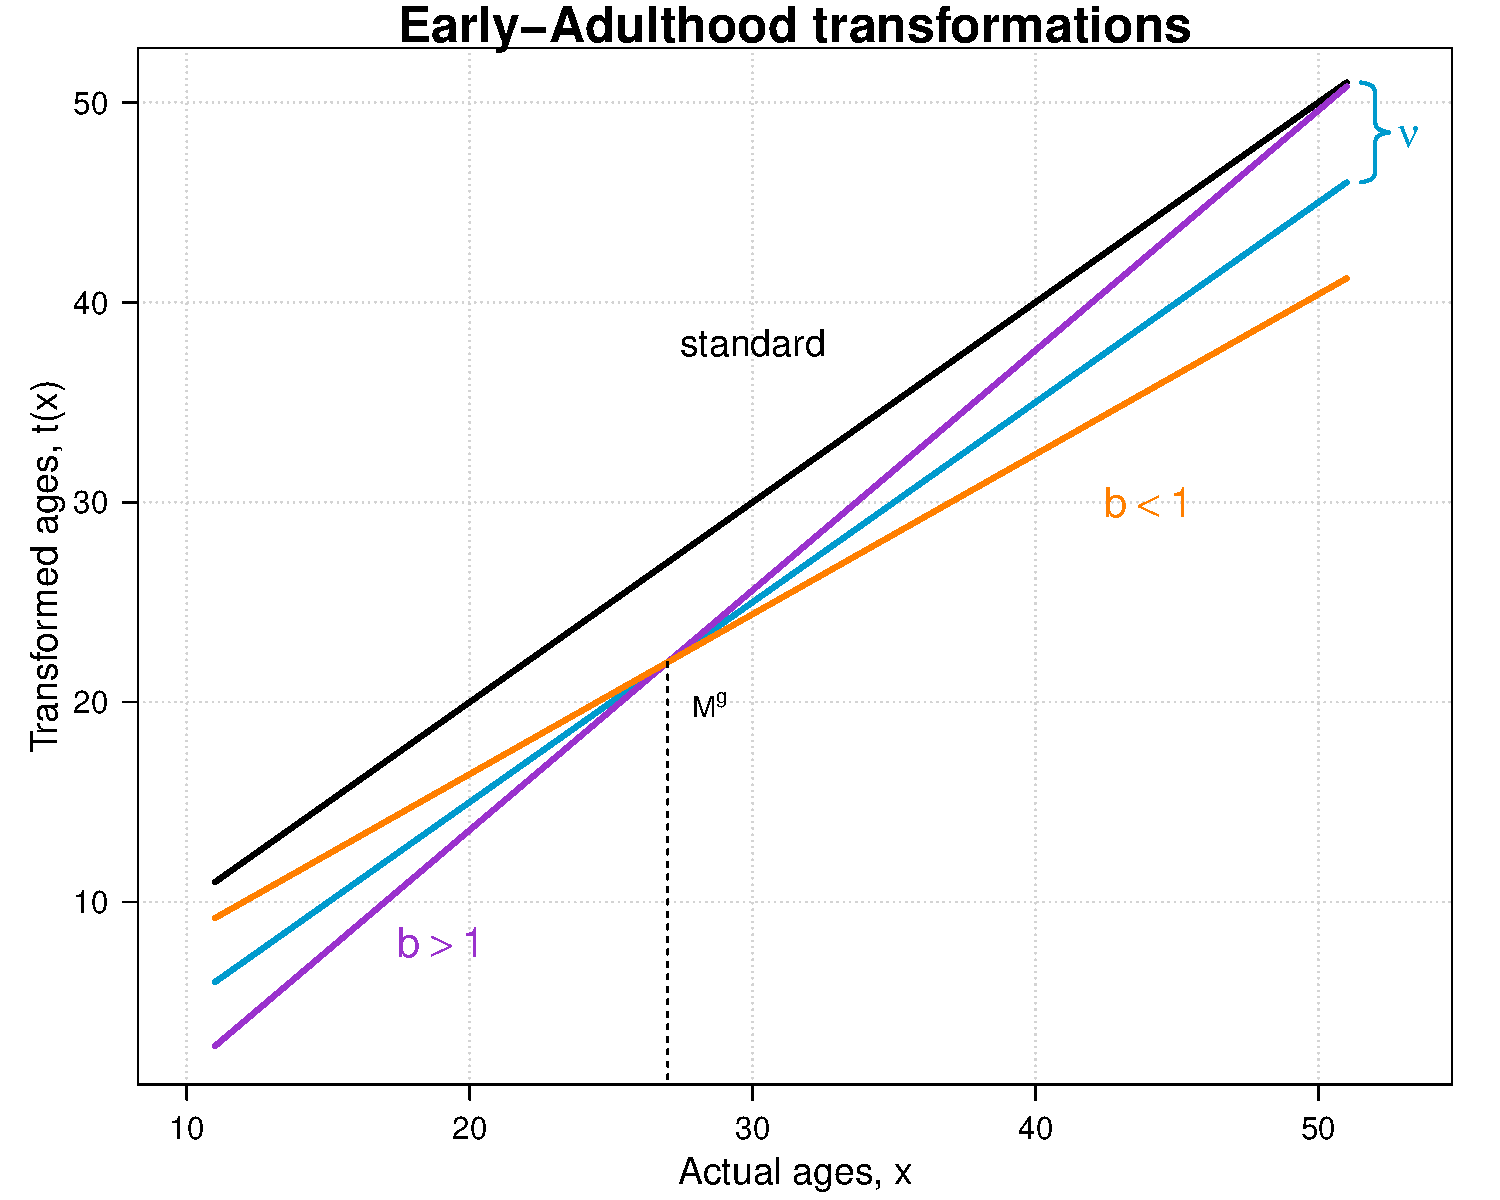
\includegraphics[scale=0.32]{./Figures/F3e.pdf}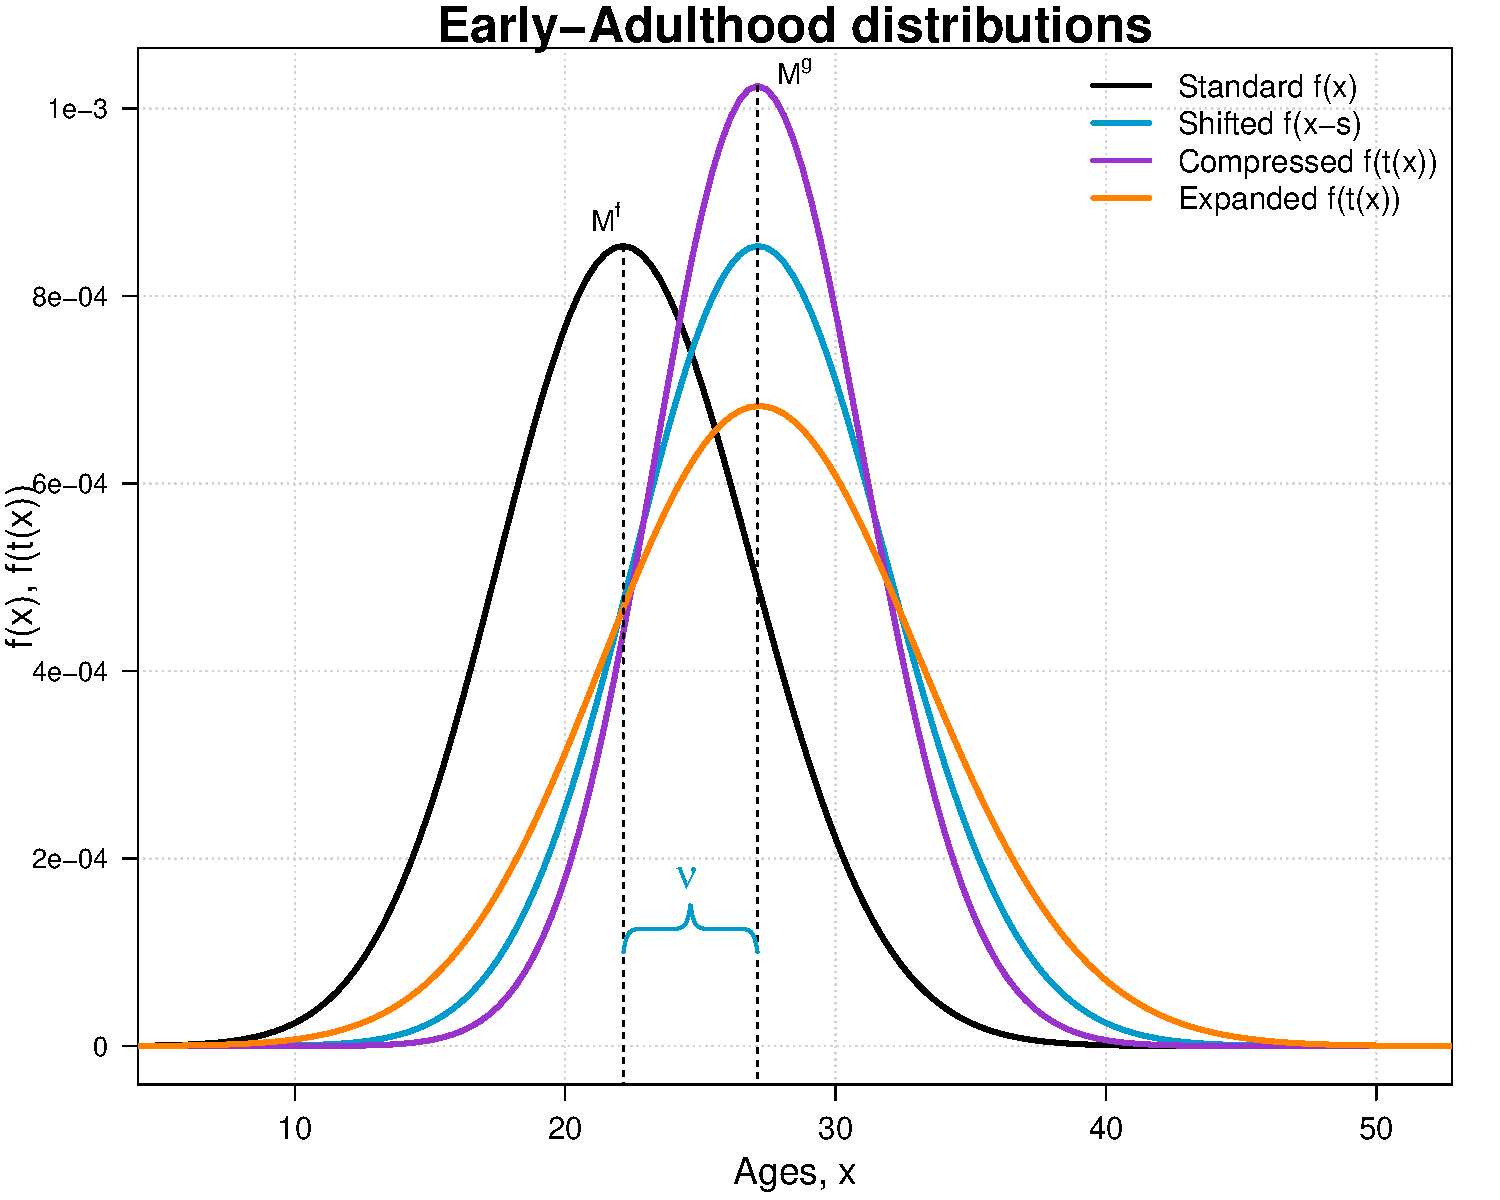
\includegraphics[scale=0.32]{./Figures/F3f.pdf}
		\caption{A graphical representation of the transformation functions (left panels) for the three components of the 3C-STAD model, and their effects on the corresponding component-specific age-at-death distributions (right panels).\\\footnotesize{\textit{Source}: authors' own elaborations.} \label{Fig:STADexample}}
	\end{center}
\end{figure}

The top panels in Figure \ref{Fig:STADexample} explain graphically the mechanisms underlying the STAD model for the Senescence component. Given a standard distribution (black lines in the graphs), let us consider the simpler case in which we vary the parameter $\nu_{s}$ but keep the {\color{red}variability} parameters equal to 1, that is, $b_{s}^{\ell} = b_{s}^{u} = 1$. The transformation function in Equation (\ref{Eq:STADsen}) then simplifies to $t_{s}(x) = x - \nu_{s}$, and the resulting distribution is shifted along the $x$-axis by an amount equal to $\nu_{s}$. This case corresponds to a shifting mortality scenario (blue lines in the graphs): the new distribution has the same shape and variability of the standard, but it is  translated by the shifting parameter.

A more general development of mortality can be described by different values of the {\color{red}variability} parameters, which act jointly with $\nu_{s}$ to modify the age-pattern of the standard distribution. When the two parameters are greater (lower) than 1, the variability of the segmented distribution is {\color{red}compressed} (expanded) before and after the modal age at death with respect to the standard. In the top right panel of Figure \ref{Fig:STADexample}, the segmented distribution has a lower variability ($b_{s}^{\ell} > 1$) before the mode and a higher variability ($b_{s}^{u} < 1$) above the mode as compared to the standard distribution. As such, {\color{red}increases in} the two parameters capture the compression dynamic of mortality, distinguishing between changes that occur before and after the modal age at death.

\subsubsection{Childhood mortality}

The modal age at death for the Childhood component is invariably at age 0. The STAD is thus simplified and we drop from the transformation in \eqref{Eq:STADsen} the part below the mode, i.e., we consider a left-truncated distribution with a constant mode at age 0. For the Childhood component, changes between the standard distribution, $f_{c}(x)$, and any observed distributions, $g_{c}(x)$, are modelled by varying the slope of the associated transformation of the age axis. In formulas, since $M_{c}^{g} = M_{c}^{f} = 0$, we can express the transformation of the age-axis as:
\begin{equation}\label{Eq:STADchil}
t_{c}(x;\;b_{c}^{u}) =  b_{c}^{u} \, x \,.
\end{equation}

The parameter $b_{c}^{u}$ captures the change in the variability of the observed (left-truncated) distribution with respect to the standard distribution. The middle panels in Figure \ref{Fig:STADexample} present this case. A parameter $b_{c}^{u}$ larger than 1 will reduce the variability of the Childhood age-at-death distribution with respect to the standard one (purple lines). Vice versa, a slope smaller than 1 will lead to an increase of the variance of the associated distribution (orange lines). 

\subsubsection{Early-adulthood mortality}

{\color{red} The Early-adulthood component of mortality is a typical and distinguishable feature of the human mortality pattern, which has been observed and modelled since the very first approaches to mortality decomposition \cite[e.g.~][]{thiele1871mathematical,lexis1878duree,pearson1897chances}. Cause-of-death investigations of young excess mortality have often provided relevant policy recommendations \citep{heuveline2002international,remund2018young}. As such, including this mortality component enhances the plausibility of fitted and forecast age-profiles, while improving the goodness-of-fit of the 3C-STAD model.}

Transformations for the Early-adulthood component account for changes in the component-specific modal age-at-death and for the variability of the observed distribution, $g_{e}(x)$, always with respect to the standard one, $f_{e}(x)$. Unlike the original STAD model, a linear transformation of the age axis without segmentation has been proven adequate for describing changes of the Early-adulthood component over years. Therefore we do not differentiate between variability before and after the mode. This adaptation of the STAD can be thought as an Accelerated Failure Time model for age-at-death distributions, where the aging process is first shifted and then uniformly accelerated/decelerated with respect to the standard distribution. 

Formally, we can write the transformation function for the Early-adulthood component as:
%
\begin{equation}\label{Eq:STADacc}
t_{e}(x;\;\nu_{e}, b_{e}) =  M_{e}^{f} + b_{e} \, \tilde{x} 
\end{equation} 
%
where $\tilde{x} = x - \nu_{e} - M_{e}^{f}$, $\nu_{e} = M_{e}^{g} - M_{e}^{f}$ and the parameter $b_{e}$ captures the change in the variability of the observed distribution $g_{e}(x)$ with respect to the standard $f_{e}(x)$. Bottom panels in Figure~\ref{Fig:STADexample} illustrates the effect of $t_{e}(\cdot)$ on a theoretical standard distribution. A shifting mortality scenario for Early-adulthood could be achieved by different values of the parameter $\nu_{e}$, keeping $b_{e}=1$ (blue lines). Alternatively, a $b_{e}$ smaller than 1 leads to an increase of the variability of the distribution, simultaneously before and after the observed mode (orange lines). A shrinkage of the age axis is achieved by a $b_{e}$ larger than 1, and it prompts a $g(x)$ with lower variability with respect to the standard $f_{e}(x)$ (purple lines). 


%%%%%%%%%%%%%%%%%%%%%%%%%%%%%%%%%%----------------------------%%%%%%%%%%%%%%%%%%%%%%%%%%%%%%%%%%----------------------------

\subsection{Estimating and forecasting the 3C-STAD parameters}\label{Subsec:STADforecast}

Being equipped with the component-specific transformation functions, we can move from the theoretical description of the 3C-STAD model to its actual application for modelling and forecasting a series of age-at-death distributions over time. The first step needed to achieve this goal is the choice of the standard distribution $f_{k}(x)$ for each component. For the Senescent component, {\color{red}we start by aligning the observed distributions to a common modal age at death, using a landmark registration approach frequently employed in Functional Data Analysis \citep{ramsay2005FDA}. The alignment procedure corresponds to a plain shifting transformation of the observed densities, which preserve all their features except the modal value. The standard is then computed as the mean of the aligned distributions. This approach increases the representativeness of the standard, which does} not conflate features of the distributions that occur at different distances with respect to the mode \cite[{\color{red}for additional details and an explicative illustration,} see][{\color{red}pp.~122--124}]{basellini2019stad}. For the Childhood and Early-adulthood components, we choose the standard as simple means of the observed distributions, as the alignment procedure is not required for the former, and it does not significantly improve the fit for the latter. 

\begin{table}[t]
	\centering
	\begin{tabular}{l|l|c|c|l}
		\multicolumn{1}{c|}{}                                & \multicolumn{1}{c|}{}                                                 & \multicolumn{2}{c|}{Parameters}         & \multicolumn{1}{c}{}                                  \\
		\multicolumn{1}{l|}{\multirow{-2}{*}{Component, $k$}} & \multicolumn{1}{l|}{\multirow{-2}{*}{Transformation, $t_{k}(\cdot)$}} & Shift     & {\color{red}Variability} & \multicolumn{1}{l}{\multirow{-2}{*}{Standard, $f_{k}(x)$}} \\ \midrule 
		\rowcolor{my-grey}  
		Senescence                                           & Segmented at the mode                                                 & $\nu_{s}$ & $b_{s}^{\ell},\,b_{s}^{u}$  & Mean of aligned distr.                                \\
		Childhood                                            & Left-Truncated, no shift                                              & --        & $b_{c}^{u}$                 & Mean of distr.                                        \\
		\rowcolor{my-grey} 
		Early-adulthood $\;$                                          & Linear, shift at the mode $\;$                                            & $\nu_{e}$ & $b_{e}$                     & Mean of distr.       \\ 
		
		\bottomrule                                  
	\end{tabular}
	\caption{Summary of the 3C-STAD model by component: type of transformation of the age axis, associated parameters and choice of the standard distribution.}\label{Table:Model}
\end{table}

Table~\ref{Table:Model} summarizes all hypotheses made in the 3C-STAD model about each component, and the associated parameters that are necessary to estimate and forecast. Given the component-specific standard distributions, parameters of the transformation functions $t_{k}(\cdot)$ are estimated from the data by maximum likelihood. Here we make use of the outcomes of the SSE model (cf.~Subsection \ref{Subsec:DataMortDecomp}), and expected number of deaths over age and time due to each component $k$, $d^{k}_{x,t}$ are modelled by the 3C-STAD. Given the actual exposures $e_{x,t}$ and assuming that component-specific expected deaths are Poisson distributed counts as in \eqref{Eq:Poisson}, we maximize the following log-likelihood function for each year $t$:
% 
\begin{equation}\label{Eq:PoiLogLike}
\ln \, \mathcal{L}\left(\bm{\theta}_{k,t}\,|\, d^{k}_{x,t} , e_{x,t} , \nu_{k,t} \right) \propto \sum_{x} \left[  d^{k}_{x,t} \,
\ln \left ( \hat{\mu}^{k}_{x,t}  \right ) - e_{x,t}
\, \hat{\mu}^{k}_{x,t}  \right]  \,, \quad k=c,a,s 
\end{equation}
%
where $\hat{\mu}^{k}_{x,t}$ denotes the hazard of component $k$ corresponding to the transformed distribution derived from $t_{k}(\cdot)$ applied in year $t$ to the associated standard $f_{k}(x)$. {\color{red}In particular, the hazard $\hat{\mu}^k_{x,t}$ is derived from the age-at-death distribution $f_{k}(t_k(\cdot))$ using standard life-table formulas \citep{preston2001demogr}.\footnote{{\color{red}One readily implemented approach to derive the hazard from age-at-death distribution in \texttt{R} is provided by the function \texttt{convertFx} in the \texttt{MortalityLaws} package  \citep{pascariu2018mortalitylaws}.}}} Note that the vector $\bm{\theta}_{k,t}$ contains only the {\color{red}variability} parameter(s). For each year $t$, the shifting parameters $\nu_{s}$ and $\nu_{e}$ of the Senescent and Early-adulthood components are computed as differences in the modal age at death between standard and observed distributions, as estimated by the SSE model. 

Once the parameters have been estimated over all years $t$, we can model their trends using standard time-series methods. Mortality forecasts of the 3C-STAD model are then obtained by extrapolating the model's parameters and the time-fixed standard distributions. We combine univariate and multivariate approaches to achieve our goal. For the Senescent component, we employ the best fitting ARIMA($p$,$d$,$q$) model for $\nu_{s}$, and a VAR(1) model for $b^{\ell}_{s}$ and $b^{u}_{s}$ \cite[as in][]{basellini2019stad}. For the Childhood component, the parameter $b_{c}^{u}$ is modelled with the best fitting ARIMA($p$,$d$,$q$) model, while for the Early-adulthood parameters $\nu_{e}$ and $b_{e}$ we employ a VAR(1) model.

The 3C-STAD acts directly on age-at-death distributions, therefore we must ensure that the sum over ages $x$ of the three component-specific probability masses is equal to 1, that is:
%
\begin{equation}\label{Eq:Masses}
\sum_{x} f_{x,t} = \sum_{x} \left( f^{c}_{x,t}+f^{e}_{x,t}+f^{s}_{x,t}  \right) = 1
\end{equation}
% 
for each year $t$. Consequently and in addition to the shifting/{\color{red}variability} parameters, it is necessary to forecast the probability masses of the three components. Specifically, we recognize the compositional nature of a set of component-specific age-at-death distributions: we are dealing with three non-negative components that always sum to a constant. We thus employ a Compositional Data methodology to model and forecast the time series of component-specific probability masses \citep{aitchison1986statistical, CoDa2011}. Specifically, we transform the probability masses for each component obtained by the SSE model using an additive log-ratio transformation. This procedure produces two time-series that are unconstrained (i.e.~they take values on the entire set of real numbers). The two transformed time-series are modelled and forecast with a VAR(1). We finally back-transform the results to obtain forecasts of the original time-series. For each forecast year, these back-transformed series sum up to 1 because they have been treated as compositional data. Note that this approach reduces the dimensionality of the forecasting problem for the probability masses by one dimension, i.e.~from three to two time-series.

Finally, the complexity of our methodology requires a bootstrapping procedure to produce prediction intervals \citep[PI,][]{efron1994introduction}. We take into account the uncertainty of the 3C-STAD parameters by simulating {\color{red}1000} new time-series of all parameters from randomly resampled residual values. For each simulation, we then forecast mortality patterns and associated summary measures. From the obtained distribution of forecast simulations, we took the median as central forecast, and the lowest and highest deciles to construct 80\% PI. Residual bootstrap of this type has already been employed to construct PI in mortality models \citep{bergeron2017coherent, basellini2019stad}.

Routines for estimating and forecasting the parameters of the 3C-STAD model were implemented in \texttt{R} \citep{Rcite} and are available online\footnote{\texttt{R} codes to replicate all results presented in this chapter are available at [the GitHub repository will be made public upon eventual acceptance of the chapter]}. Our routines take advantage of the \texttt{R} packages \texttt{forecast}, \texttt{demography}, \texttt{MortalitySmooth}, {\color{red}\texttt{MortalityLaws}} and \texttt{vars} \citep{pfaff2008analysis,pfaff2008var,hyndman2008automatic,camarda2012mortalitysmooth,hyndman2018forecastR,demogRpackage,pascariu2018mortalitylaws}.  

%%%%%%%%%%%%%%%%%%%%%%%%%%%%%%%%%%----------------------------%%%%%%%%%%%%%%%%%%%%%%%%%%%%%%%%%%----------------------------

\section{Results}\label{Sec:Results}

%%%%%%%%%%%%%%%%%%%%%%%%%%%%%%%%%%----------------------------%%%%%%%%%%%%%%%%%%%%%%%%%%%%%%%%%%----------------------------

\subsection{Out-of-sample validation}\label{Subsec:OutOfSample}

Here, we assess the predictive performance of the 3C-STAD model using out-of-sample validation. Specifically, we employ data of the \cite{HMD} for the female and male populations of Sweden and Switzerland for the period 1950-2016. For each population, we perform three exercises, corresponding to validation periods of 10 years (training period 1950-2006), 20 years (training period 1950-1996) and 30 years (training period 1950-1986). The common starting year of analysis, 1950, was chosen in order to have training periods longer than validation horizons for each exercise. 

To assess the performance of our forecasts, we employ the standard life-table functions: life expectancy at birth ($e_{t}^{0}$) as measure of population's longevity in year $t$, and age-specific mortality rates (in log scale, $\ln(m_{x,t})$), which measure the age-pattern and intensity of mortality. Additionally, we use the Gini coefficient ($g^{0}_{t}$), a measure of lifespan inequality, whose importance for evaluating mortality forecasts has been recently highlighted \citep{bohk2017lifespan}. 

We compare the performance accuracy of the 3C-STAD model with three other forecasting methodologies. First, given its prominence and wide application, we employ the original model of \citeauthor{lee1992modeling} (LC, \citeyear{lee1992modeling}). Second, since one limitation of the LC model is the lack of smoothness in the fitted and forecast mortality rates, we use the functional data model of \citeauthor{hyndman2007robust} (HU, \citeyear{hyndman2007robust}), which overcomes this limitation by smoothing the starting data as a first step. Third, we choose the CODA model proposed by \cite{oeppen2008coherent}: this model is indeed closer in spirit to the 3C-STAD, as it models and forecasts the age-at-death distribution. The LC and HU models were estimated and forecast with the \texttt{R} packages \texttt{forecast} and \texttt{demography} \citep{hyndman2018forecastR,demogRpackage,hyndman2008automatic}. The CODA model was fitted and forecast using the \texttt{R} codes provided in the Supplementary Material of \cite{bergeron2017coherent}. 

Our evaluations of mortality forecasts are based on the accuracy of both point predictions and calibration of prediction intervals (PI), as both measures are relevant for the validation of probabilistic projections \citep{chatfield2000time}. Greater accuracy in point forecasts occurs when point predictions are closer to the observed data. To evaluate point forecasts, we employ the mean absolute error (MAE), which is defined as:
%
\begin{equation}\label{Eq:MAE}
	\mathrm{MAE} = \frac{1}{N} \sum_{t \in T} \left| \hat{y_t} - y_t \right|  \notag 
\end{equation}
% 
where $\hat{y_t}$ is the point forecast at time $t$ for either life expectancy at birth, mortality rates or Gini coefficient. Associated out-of-sample observed values are denoted by $y_t$. The set of validation years is $T$, and $N$ is the total number of data used for validation. Note that for mortality rates, mean is computed over ages, too. 

Greater calibration of PI is achieved when the proportion of out-of-sample data that falls within the calculated PI is closer to the given nominal level (for example, 80\% or 95\%). To evaluate interval forecasts, we compute the empirical coverage probability (ECP) of the 80\% PI for each model \cite[as in, for example,][]{shang2011point,raftery2013bayesian}. For the sake of consistency and fairness, we computed the PI for all models by the same bootstrapping procedure, i.e.~residual bootstrap of the time-series of the model's parameters (cf.~Subsection \ref{Subsec:STADforecast}).

{\color{red}In addition to the MAE and ECP, proper scoring rules can be used to assess calibration and sharpness of probabilistic forecasts simultaneously \cite[for a review, see][]{gneiting2014probabilistic}. Scoring rules allow to jointly assess point and interval predictions by providing a summary measure of the predictive performance that forecasters aim to minimize. Here, we employ the proper Dawid-Sebastiani score (DSS) \citep{dawid1999coherent}, which is given by:
%
\begin{equation}\label{Eq:DSS}
\mathrm{DSS}_t = \frac{\left(y_t-\mu_{F,t}\right)^2}{\sigma^2_{F,t}} + 2 \ln \sigma_{F,t}  \,, \quad t \in T \notag 
\end{equation}
%
where $\mu_{F,t}$ and $\sigma^2_{F,t}$ are the first two central moments of the probabilistic forecast at time $t$, $y_t$ is the associated out-of-sample observed value, and $T$ is the set of validation years. We then compute the mean value of the DSS for all the data used for validation. 
}

Table \ref{Table:Validation} reports the point, interval and {\color{red}probabilistic} forecast accuracy of the four models in the three out-of-sample scenarios as well as for all the four populations analysed here. Bold values correspond to better performances. In terms of point forecast, the 3C-STAD is the most accurate model, as its forecasts are more or as precise as those of the other models. Out of 36 indicators, the 3C-STAD outperforms 20 times. The HU is the second most precise model with {\color{red}9} indicators, followed by the LC and CODA models, each with {\color{red}8} and 3 indicators, respectively. Note that the sum does not add up to the total number of indicators due to the draw of some models for some specific measures {\color{red}(for example, both the 3C-STAD and LC models are equally best performers for the indicator $g^0$ for Swedish females in the 30y exercise)}. In terms of interval forecast, the CODA outperforms all other models, being more accurate for 15 indicators over 36. The 3C-STAD, {\color{red}LC} and HU follow, each with {\color{red}12, 11 and 7} indicators, respectively. {\color{red}Finally, if we consider point and prediction accuracy simultaneously using the DSS measure, we find that the HU and 3C-STAD models are the best performer, each one outperforming the others for 12 and 11 indicators, respectively. The LC model follows with 9, while the CODA is the best performer for only 4 indicators.} 

%%%%%%%%%%%%%%%%%%%%%%%%%%%%%%%%%%----------------------------%%%%%%%%%%%%%%%%%%%%%%%%%%%%%%%%%%----------------------------

\subsection{Forecast to 2050}\label{Subsec:Forecast2050}

Having assessed and compared the forecast accuracy of the 3C-STAD model, we now present its mortality forecasts for the four populations analysed until 2050. As in the previous Subsection, we compare projections based on the 3C-STAD model with those of LC, HU and CODA models.

Figure \ref{Fig:e0g0fore} shows the observed and forecast life expectancy at birth ($e^{0}$) and Gini coefficient ($g^{0}$) in the four populations for the years 1950-2050. In terms of $e^{0}$, the 3C-STAD forecasts are always more optimistic than those of the LC and HU model. With respect to CODA, the 3C-STAD is more optimistic for males and less optimistic for females. In terms of lifespan inequality, CODA forecasts are the most egalitarian in 2050 (lower values of $g^{0}$) for the female populations, while the 3C-STAD predicts more equality for males.

In Figure \ref{Fig:LMXfore}, we compare the age-specific mortality rates forecasts in 2050 for all populations. Several differences emerge between the models from this age-pattern analysis. Mortality rates of the 3C-STAD are smooth, lacking the jagged features visible in the LC and CODA forecasts. This is a great advantage for long-term mortality projections \citep{li2013extending}. Additionally, the Swedish projections of the 3C-STAD do not display an unexpected S-shape displayed by other models in the age range 60-100. 

Finally, Figure \ref{Fig:DXfore} shows the observed age-at-death distribution for the four populations in 2016, along with the 2050 forecasts of the four models. With respect to the other models, the 3C-STAD forecasts are characterized by greatest shift for all the populations. In addition to this, the 3C-STAD projections are also less compressed than those of other models, with the exception of Swedish males.


%%%%%%%%%%%%%%%%%%%%%%%%%%%%%%%%%%----------------------------%%%%%%%%%%%%%%%%%%%%%%%%%%%%%%%%%%----------------------------
%%%%%%%%%%%%%%%%%%%%%%%%%%%%%%%%%%    TABLE AND FIGURES       %%%%%%%%%%%%%%%%%%%%%%%%%%%%%%%%%%----------------------------
%%%%%%%%%%%%%%%%%%%%%%%%%%%%%%%%%%----------------------------%%%%%%%%%%%%%%%%%%%%%%%%%%%%%%%%%%----------------------------

\begin{landscape}
	% TABLE TOTAL: 10, 20, 30 YEARS
	\begin{table}[h!]
	\centering
	\scriptsize
	\begin{tabular}{lC{1.3cm}C{1.3cm}cC{1cm}|C{1cm}|C{1cm}|C{1cm}|C{1cm}|C{1cm}|C{1cm}|C{1cm}|C{1cm}|C{1cm}|C{1cm}|C{1cm}}
	\toprule & & & & \multicolumn{12}{c}{\textbf{Forecast Accuracy}} \\ \cmidrule{5-16} 
	& & &  &  \multicolumn{4}{c}{\textbf{Point forecast }(MAE)}    & \multicolumn{4}{c}{\textbf{Interval forecast} (ECP for 80\% PI)} 
	& \multicolumn{4}{c}{{\color{red}\textbf{Probabilistic forecast} (mean DSS)}} \\ 
	\cmidrule{5-16} Country $\quad$ & Training period & Validation period &   Measure  &  3C-STAD & LC & CODA & HU & 3C-STAD & LC & CODA & HU & {\color{red}3C-STAD} & {\color{red}LC} & {\color{red}CODA} & {\color{red}HU}  \\
	\midrule
				
	%%% CHE Females %%% CHE Females %%% CHE Females
	%%% CHE Females %%% CHE Females %%% CHE Females
				
	\rowcolor{my-grey} 
	\multicolumn{1}{l|}{\cellcolor{my-grey}}    &  \multicolumn{1}{c|}{\cellcolor{my-grey}} &  \multicolumn{1}{c|}{\cellcolor{my-grey}}  & \multicolumn{1}{c|}{\cellcolor{my-grey}$e^{0}$} & \textbf{0.11}  & 0.29   & 0.40  & 0.16   & 100\% & 100\% & 100\% & \textbf{90\%} & 1.10  &  1.40  &  1.61 & \textbf{1.08} \\
	\rowcolor{my-grey} 
	\multicolumn{1}{l|}{\cellcolor{my-grey}}    &  \multicolumn{1}{c|}{\cellcolor{my-grey}} & \multicolumn{1}{c|}{\cellcolor{my-grey}} & \multicolumn{1}{c|}{\cellcolor{my-grey}$g^{0}$} & 0.08 & 0.11   & 0.09 & \textbf{0.06}   & 100\% &  \textbf{80\%}  & 90\% & \textbf{80\%}  & 0.92  &  1.13 &    \textbf{0.71} & 1.12   \\
	\rowcolor{my-grey} 
	\multicolumn{1}{l|}{\cellcolor{my-grey}} & \multicolumn{1}{c|}{\multirow{-3}{*}{\cellcolor{my-grey}1950-2006}} &  \multicolumn{1}{c|}{\multirow{-3}{*}{\cellcolor{my-grey}10y}} & \multicolumn{1}{c|}{\cellcolor{my-grey}$\ln(m_{x,t})$}      & \textbf{0.19} & 0.24  & 0.24  & 0.22   & 38\% & 35\% & \textbf{47\%} & 37\% & 25.25 & 40.51 & 74.56 & \textbf{11.61} \\ 
	\hhline{~|---------------|}
	\rowcolor{my-white} 
	\multicolumn{1}{l|}{\cellcolor{my-grey}}    & \multicolumn{1}{c|}{\cellcolor{my-white}} & \multicolumn{1}{c|}{\cellcolor{my-white}}  & \multicolumn{1}{c|}{\cellcolor{my-white}$e^{0}$} & 0.13  & 0.11   & 0.39  &  \textbf{0.12}   & 100\% & 100\% & 100\% & \textbf{95\%} & 1.69  &   1.65 &   1.70 &  \textbf{0.91} \\
	\rowcolor{my-white} 
	\multicolumn{1}{l|}{\cellcolor{my-grey}}    & \multicolumn{1}{c|}{\cellcolor{my-white}} & \multicolumn{1}{c|}{\cellcolor{my-white}} & \multicolumn{1}{c|}{\cellcolor{my-white}$g^{0}$} & 0.08  & \textbf{0.06} & 0.21  & 0.10 & 90\% & 100\% & 95\% & \textbf{85\%} & 0.97 &   \textbf{0.63} & 1.22 & 1.34 \\
	\rowcolor{my-white} 
	\multicolumn{1}{l|}{\cellcolor{my-grey}} & \multicolumn{1}{c|}{\multirow{-3}{*}{\cellcolor{my-white}{1950-1996}}} & \multicolumn{1}{c|}{\multirow{-3}{*}{\cellcolor{my-white}{20y}}} & \multicolumn{1}{c|}{\cellcolor{my-white}$\ln(m_{x,t})$}      & \textbf{0.19} & 0.24  & 0.23 & 0.23   & 51\% & 48\% & \textbf{54\%} & 38\% & 15.13  & 48.47 & 32.40 & \textbf{10.13}  \\ 
	\hhline{~|---------------|}
	\rowcolor{my-grey} 
	\multicolumn{1}{l|}{\cellcolor{my-grey}}    &  \multicolumn{1}{c|}{\cellcolor{my-grey}} & \multicolumn{1}{c|}{\cellcolor{my-grey}} & \multicolumn{1}{c|}{\cellcolor{my-grey}$e^{0}$} & 0.74 & 0.43  & 0.45  & \textbf{0.20}   & \textbf{87\%} & 100\% & 97\% & 93\% & 2.48 &   2.18  & 1.75 & \textbf{1.44}    \\
	\rowcolor{my-grey} 
	\multicolumn{1}{l|}{\cellcolor{my-grey}}    &  \multicolumn{1}{c|}{\cellcolor{my-grey}} & \multicolumn{1}{c|}{\cellcolor{my-grey}} & \multicolumn{1}{c|}{\cellcolor{my-grey}$g^{0}$} & 0.21 & 0.40 & 0.30 & \textbf{0.13} & 70\%   & 63\% &  37\%  & \textbf{77\%}  & 2.54  &  2.96  & 2.43  & \textbf{1.30}  \\
	\rowcolor{my-grey} 
	\multicolumn{1}{l|}{\multirow{-9}{*}{\cellcolor{my-grey}\thead{Switzerland \\ Females}}} & \multicolumn{1}{c|}{\multirow{-3}{*}{\cellcolor{my-grey}1950-1986}} & \multicolumn{1}{c|}{\multirow{-3}{*}{\cellcolor{my-grey}30y}} & \multicolumn{1}{c|}{\cellcolor{my-grey}$\ln(m_{x,t})$}      & 0.22 & 0.28   & 0.23 & \textbf{0.20} & 54\% & 50\% & \textbf{58\%}  & 43\% & 12.16 & 20.08 & 22.54 & \textbf{8.00}  \\ 	\midrule
	
	%% CHE Males
	
	\rowcolor{my-white} 
	\multicolumn{1}{l|}{\cellcolor{my-white}}    &     \multicolumn{1}{c|}{\cellcolor{my-white}}  & \multicolumn{1}{c|}{\cellcolor{my-white}}  & \multicolumn{1}{c|}{\cellcolor{my-white}$e^{0}$} & \textbf{0.19} & 0.41  & 0.34  & 0.78   & 100\% & \textbf{90\%} & 100\% & 0\% & \textbf{1.17}  &  1.70 &  1.84 &  6.95  \\
	\rowcolor{my-white} 
	\multicolumn{1}{l|}{\cellcolor{my-white}}    &     \multicolumn{1}{c|}{\cellcolor{my-white}}                 & \multicolumn{1}{c|}{\cellcolor{my-white}}    & \multicolumn{1}{c|}{\cellcolor{my-white}$g^{0}$} & 0.13  & 0.21  & \textbf{0.12}  & 0.26   & \textbf{80\%} & 70\% & 100\% & 10\% & 1.15  &  1.84  & \textbf{0.85} & 5.83  \\
	\rowcolor{my-white} 
	\multicolumn{1}{l|}{\cellcolor{my-white}} & \multicolumn{1}{c|}{\multirow{-3}{*}{\cellcolor{my-white}1950-2006}} & \multicolumn{1}{c|}{\multirow{-3}{*}{\cellcolor{my-white}10y}} & \multicolumn{1}{c|}{\cellcolor{my-white}$\ln(m_{x,t})$} & \textbf{0.17}   & 0.23  & 0.20 &  0.20   & 37\% & 32\% & \textbf{53\%} & 31\% & 13.70  &  39.52 & 53.54 & \textbf{8.54}  \\ 
	\hhline{~|---------------|}
	\rowcolor{my-grey} 
	\multicolumn{1}{l|}{\cellcolor{my-white}}    &         \multicolumn{1}{c|}{\cellcolor{my-grey}}             & \multicolumn{1}{c|}{\cellcolor{my-grey}}    & \multicolumn{1}{c|}{\cellcolor{my-grey}$e^{0}$} & \textbf{1.39} & 1.59  & 1.61 & 2.23  & 10\% & 20\%  & \textbf{25\%} & 0\% & 5.09   & 5.31 &  \textbf{4.80} &  46.32    \\
	\rowcolor{my-grey} 
	\multicolumn{1}{l|}{\cellcolor{my-white}}    &      \multicolumn{1}{c|}{\cellcolor{my-grey}}    & \multicolumn{1}{c|}{\cellcolor{my-grey}}   & \multicolumn{1}{c|}{\cellcolor{my-grey}$g^{0}$} & \textbf{0.46} & 0.74  & 0.65 & 1.01   & 15\% & 0\%  & \textbf{20\%} & 0\% & \textbf{4.45}  &  9.83  & 4.49 & 56.09  \\
	\rowcolor{my-grey} 
	\multicolumn{1}{l|}{\cellcolor{my-white}} & \multicolumn{1}{c|}{\multirow{-3}{*}{\cellcolor{my-grey}{1950-1996}}} & \multicolumn{1}{c|}{\multirow{-3}{*}{\cellcolor{my-grey}{20y}}} & \multicolumn{1}{c|}{\cellcolor{my-grey}$\ln(m_{x,t})$} & \textbf{0.25} & 0.29  & 0.28 & 0.32   & 29\% & 29\% & \textbf{43\%}  & 17\% & \textbf{20.32} &  168137 & 71.00 & 21.54 \\ 
	\hhline{~|---------------|}
	\rowcolor{my-white} 
	\multicolumn{1}{l|}{\cellcolor{my-white}}    &   \multicolumn{1}{c|}{\cellcolor{my-white}} & \multicolumn{1}{c|}{\cellcolor{my-white}} & \multicolumn{1}{c|}{\cellcolor{my-white}$e^{0}$} & \textbf{1.55} & 1.63  & 2.27  & 1.94  & 37\% & \textbf{47\%} & 30\% & 17\% & 6.17 &   \textbf{4.52} & 6.23 &  34.29 \\
	\rowcolor{my-white} 
	\multicolumn{1}{l|}{\cellcolor{my-white}}    &  \multicolumn{1}{c|}{\cellcolor{my-white}}  & \multicolumn{1}{c|}{\cellcolor{my-white}}  & \multicolumn{1}{c|}{\cellcolor{my-white}$g^{0}$} & 0.98 & \textbf{0.64} &  0.88  & 0.71  & 20\% & \textbf{27\%} & \textbf{27\%} & 17\% & 6.05  &  \textbf{4.72} &  6.07 & 43.39  \\
	\rowcolor{my-white} 
	\multicolumn{1}{l|}{\multirow{-9}{*}{\cellcolor{my-white}\thead{Switzerland \\ Males}}} & \multicolumn{1}{c|}{\multirow{-3}{*}{\cellcolor{my-white}1950-1986}} & \multicolumn{1}{c|}{\multirow{-3}{*}{\cellcolor{my-white}30y}} & \multicolumn{1}{c|}{\cellcolor{my-white}$\ln(m_{x,t})$} & 0.31 & \textbf{0.27} & 0.31 & \textbf{0.27} & 25\% & 35\% & \textbf{42\%} & 21\% & \textbf{19.86} &   103.94 & 22.85 & 23.81  \\ \midrule
	
	%% SWE Females %% SWE Females %% SWE Females
	%% SWE Females %% SWE Females %% SWE Females
	
	\rowcolor{my-grey} 
	\multicolumn{1}{l|}{\cellcolor{my-grey}}    &  \multicolumn{1}{c|}{\cellcolor{my-grey}} &  \multicolumn{1}{c|}{\cellcolor{my-grey}}  & \multicolumn{1}{c|}{\cellcolor{my-grey}$e^{0}$} & 0.12   & \textbf{0.10}    & 0.38   & 0.15  & \textbf{100\%} & \textbf{100\%} & \textbf{100\%} & \textbf{100\%} & \textbf{0.82}  &  0.99 &  1.66 & 0.99 \\
	\rowcolor{my-grey} 
	\multicolumn{1}{l|}{\cellcolor{my-grey}}    &  \multicolumn{1}{c|}{\cellcolor{my-grey}} & \multicolumn{1}{c|}{\cellcolor{my-grey}} & \multicolumn{1}{c|}{\cellcolor{my-grey}$g^{0}$} & 0.07   & \textbf{0.05}    & 0.13  & 0.12   & \textbf{80\%} & 90\% & 100\% & 50\% & 1.30  & \textbf{0.70}  & 0.82 &  2.93    \\
	\rowcolor{my-grey} 
	\multicolumn{1}{l|}{\cellcolor{my-grey}} & \multicolumn{1}{c|}{\multirow{-3}{*}{\cellcolor{my-grey}1950-2006}} &  \multicolumn{1}{c|}{\multirow{-3}{*}{\cellcolor{my-grey}10y}} & \multicolumn{1}{c|}{\cellcolor{my-grey}$\ln(m_{x,t})$} & \textbf{0.16}  & 0.18   & 0.22   & \textbf{0.16}   & 37\% & 39\%  & \textbf{55\%} & 44\% & 25.12 &  19.83 & 93.65 & \textbf{9.91} \\ 
	\hhline{~|---------------|}
	\rowcolor{my-white} 
	\multicolumn{1}{l|}{\cellcolor{my-grey}}    & \multicolumn{1}{c|}{\cellcolor{my-white}} & \multicolumn{1}{c|}{\cellcolor{my-white}}  & \multicolumn{1}{c|}{\cellcolor{my-white}$e^{0}$} & 0.46   &  \textbf{0.17}    & 0.73  & 0.46 & \textbf{90\%} & 100\% & 95\% & 20\% & 1.79  &  \textbf{1.53} &  2.42 & 2.90 \\
	\rowcolor{my-white} 
	\multicolumn{1}{l|}{\cellcolor{my-grey}}    & \multicolumn{1}{c|}{\cellcolor{my-white}} & \multicolumn{1}{c|}{\cellcolor{my-white}} & \multicolumn{1}{c|}{\cellcolor{my-white}$g^{0}$} & \textbf{0.06}  & 0.10    & 0.20   & \textbf{0.06} & 95\% & 90\% & 95\% & \textbf{85\%} & \textbf{0.65} &   1.06 &  1.16 & 0.99 \\
	\rowcolor{my-white} 
	\multicolumn{1}{l|}{\cellcolor{my-grey}} & \multicolumn{1}{c|}{\multirow{-3}{*}{\cellcolor{my-white}{1950-1996}}} & \multicolumn{1}{c|}{\multirow{-3}{*}{\cellcolor{my-white}{20y}}} & \multicolumn{1}{c|}{\cellcolor{my-white}$\ln(m_{x,t})$} & \textbf{0.18} & 0.19  & 0.22 & 0.19 & 43\% & 45\% & \textbf{54\%} & 28\% & 24.70  & \textbf{11.06} & 52.18 &  12.26 \\ 
	\hhline{~|---------------|}
	\rowcolor{my-grey} 
	\multicolumn{1}{l|}{\cellcolor{my-grey}}    &  \multicolumn{1}{c|}{\cellcolor{my-grey}} & \multicolumn{1}{c|}{\cellcolor{my-grey}} & \multicolumn{1}{c|}{\cellcolor{my-grey}$e^{0}$} & 0.69    & 0.53    & 1.43     & \textbf{0.43}   & 23\% & \textbf{97\%} & 7\% & 30\% & 3.62 &   \textbf{2.08} & 10.81 & 3.04    \\
	\rowcolor{my-grey} 
	\multicolumn{1}{l|}{\cellcolor{my-grey}}    &  \multicolumn{1}{c|}{\cellcolor{my-grey}} & \multicolumn{1}{c|}{\cellcolor{my-grey}} & \multicolumn{1}{c|}{\cellcolor{my-grey}$g^{0}$} & \textbf{0.07}  &  \textbf{0.07}    & 0.34     & 0.09   & \textbf{80\%} & 87\% & 20\% & 70\% & 1.34 &   \textbf{1.03} & 6.13 &  1.64  \\
	\rowcolor{my-grey} 
	\multicolumn{1}{c|}{\multirow{-9}{*}{\cellcolor{my-grey}\thead{Sweden \\ Females}}} & \multicolumn{1}{c|}{\multirow{-3}{*}{\cellcolor{my-grey}1950-1986}} & \multicolumn{1}{c|}{\multirow{-3}{*}{\cellcolor{my-grey}30y}} & \multicolumn{1}{c|}{\cellcolor{my-grey}$\ln(m_{x,t})$} & \textbf{0.18} & 0.21   & 0.27   & 0.19 & \textbf{39\%} & \textbf{39\%} & 34\% & 29\% & \textbf{15.92} &  33.39 & 87.08 & 16.73 \\ \midrule
	
	
	%% SWE Males %% SWE Males %% SWE Males
	%% SWE Males %% SWE Males %% SWE Males
	
	\rowcolor{my-white} 
	\multicolumn{1}{l|}{\cellcolor{my-white}}    &     \multicolumn{1}{c|}{\cellcolor{my-white}}  & \multicolumn{1}{c|}{\cellcolor{my-white}}  & \multicolumn{1}{c|}{\cellcolor{my-white}$e^{0}$} & \textbf{0.11}  & 0.38   & 0.41    & 0.81  & \textbf{100\%} & \textbf{100\%} & \textbf{100\%} & 0\% & \textbf{1.05} &   1.57 &    1.62  & 7.75  \\
	\rowcolor{my-white} 
	\multicolumn{1}{l|}{\cellcolor{my-white}}    &     \multicolumn{1}{c|}{\cellcolor{my-white}}                 & \multicolumn{1}{c|}{\cellcolor{my-white}}    & \multicolumn{1}{c|}{\cellcolor{my-white}$g^{0}$} & 0.10   & 0.09    & \textbf{0.03}  & 0.04 & \textbf{70\%} & \textbf{90\%} & 100\% & 100\% & 1.29 &   1.06 &  0.42 &  \textbf{0.38}  \\
	\rowcolor{my-white} 
	\multicolumn{1}{l|}{\cellcolor{my-white}} & \multicolumn{1}{c|}{\multirow{-3}{*}{\cellcolor{my-white}1950-2006}} & \multicolumn{1}{c|}{\multirow{-3}{*}{\cellcolor{my-white}10y}} & \multicolumn{1}{c|}{\cellcolor{my-white}$\ln(m_{x,t})$} &  \textbf{0.17}   & 0.23    &  0.19  &  0.18 & 43\% & 26\% & \textbf{49\%} & 27\% & 25.41  & 120.36 & 127.46 & \textbf{11.36}  \\ 
	\hhline{~|---------------|}
	\rowcolor{my-grey} 
	\multicolumn{1}{l|}{\cellcolor{my-white}}    &  \multicolumn{1}{c|}{\cellcolor{my-grey}}  & \multicolumn{1}{c|}{\cellcolor{my-grey}}    & \multicolumn{1}{c|}{\cellcolor{my-grey}$e^{0}$} & \textbf{0.72}   & 1.35     & 1.34   & 1.69 & \textbf{100\%} & 30\% & 15\% & 0\% & \textbf{2.61}  &  4.48 &  7.82 &  18.73  \\
	\rowcolor{my-grey} 
	\multicolumn{1}{l|}{\cellcolor{my-white}}    &      \multicolumn{1}{c|}{\cellcolor{my-grey}}    & \multicolumn{1}{c|}{\cellcolor{my-grey}}   & \multicolumn{1}{c|}{\cellcolor{my-grey}$g^{0}$} & 0.32   & 0.37     & \textbf{0.26}    & 0.39 & 15\% & 10\% & \textbf{40\%} & 0\% & 4.00  &  3.36  & \textbf{3.20}  & 5.42  \\
	\rowcolor{my-grey} 
	\multicolumn{1}{l|}{\cellcolor{my-white}} & \multicolumn{1}{c|}{\multirow{-3}{*}{\cellcolor{my-grey}{1950-1996}}} & \multicolumn{1}{c|}{\multirow{-3}{*}{\cellcolor{my-grey}{20y}}} & \multicolumn{1}{c|}{\cellcolor{my-grey}$\ln(m_{x,t})$} & \textbf{0.20} & 0.29  & 0.23 & 0.21 & \textbf{51\%} & 21\% & 32\% & 27\% & 15.73  & 120.98 & 70.90 & \textbf{12.10} \\ 
	\hhline{~|---------------|}
	\rowcolor{my-white} 
	\multicolumn{1}{l|}{\cellcolor{my-white}}    &   \multicolumn{1}{c|}{\cellcolor{my-white}} & \multicolumn{1}{c|}{\cellcolor{my-white}} & \multicolumn{1}{c|}{\cellcolor{my-white}$e^{0}$} & 2.65 & \textbf{2.43}   & 2.59    & 3.14   & 7\% & \textbf{13\%} & 7\% & 0\% & 20.92 &  \textbf{9.79} & 75.35 & 153.06 \\
	\rowcolor{my-white} 
	\multicolumn{1}{l|}{\cellcolor{my-white}}    &  \multicolumn{1}{c|}{\cellcolor{my-white}}  & \multicolumn{1}{c|}{\cellcolor{my-white}}  & \multicolumn{1}{c|}{\cellcolor{my-white}$g^{0}$} & \textbf{0.40}    & 0.83    & 0.93    & 1.02   & \textbf{23\%} & 17\% & 10\% & 10\% & \textbf{3.54} & 13.67 &  72.39 & 80.96  \\
	\rowcolor{my-white} 
	\multicolumn{1}{c|}{\multirow{-9}{*}{\cellcolor{my-white}\thead{Sweden \\ Males}}} & \multicolumn{1}{c|}{\multirow{-3}{*}{\cellcolor{my-white}1950-1986}} & \multicolumn{1}{c|}{\multirow{-3}{*}{\cellcolor{my-white}30y}} & \multicolumn{1}{c|}{\cellcolor{my-white}$\ln(m_{x,t})$} & \textbf{0.29}  & 0.38  & 0.31  & 0.31 & 18\% & \textbf{28\%} & 25\% & 16\% & \textbf{21.87} &  98.09 & 56.84 & 50.36  \\ 
	
	\bottomrule 
				
	\end{tabular}
	\caption{Mean absolute error (MAE), empirical coverage probability (ECP) for the 80\% PI, {\color{red}and mean Dawid-Sebastiani score (DSS)} of the 3C-STAD, LC, CODA and HU forecasts of $e^{0}$, $g^{0}$ and $\ln(m_{x,t})$ for females and males in two countries and three out-of-sample exercises: validation periods of 10 years (training period 1950-2006), 20 years (1950-1996) and 30 years (1950-1986). Lower values of the MAE {\color{red}and of the DSS} (in bold) correspond to greater forecast accuracy. Values of the ECP closer to the 80\% nominal level (in bold) correspond to greater interval forecast accuracy.\\\footnotesize{\textit{Source}: as for Figure \ref{Fig:Intro}.}}\label{Table:Validation}
	\end{table}

\end{landscape}

\begin{figure}[h!]
	\begin{center}
		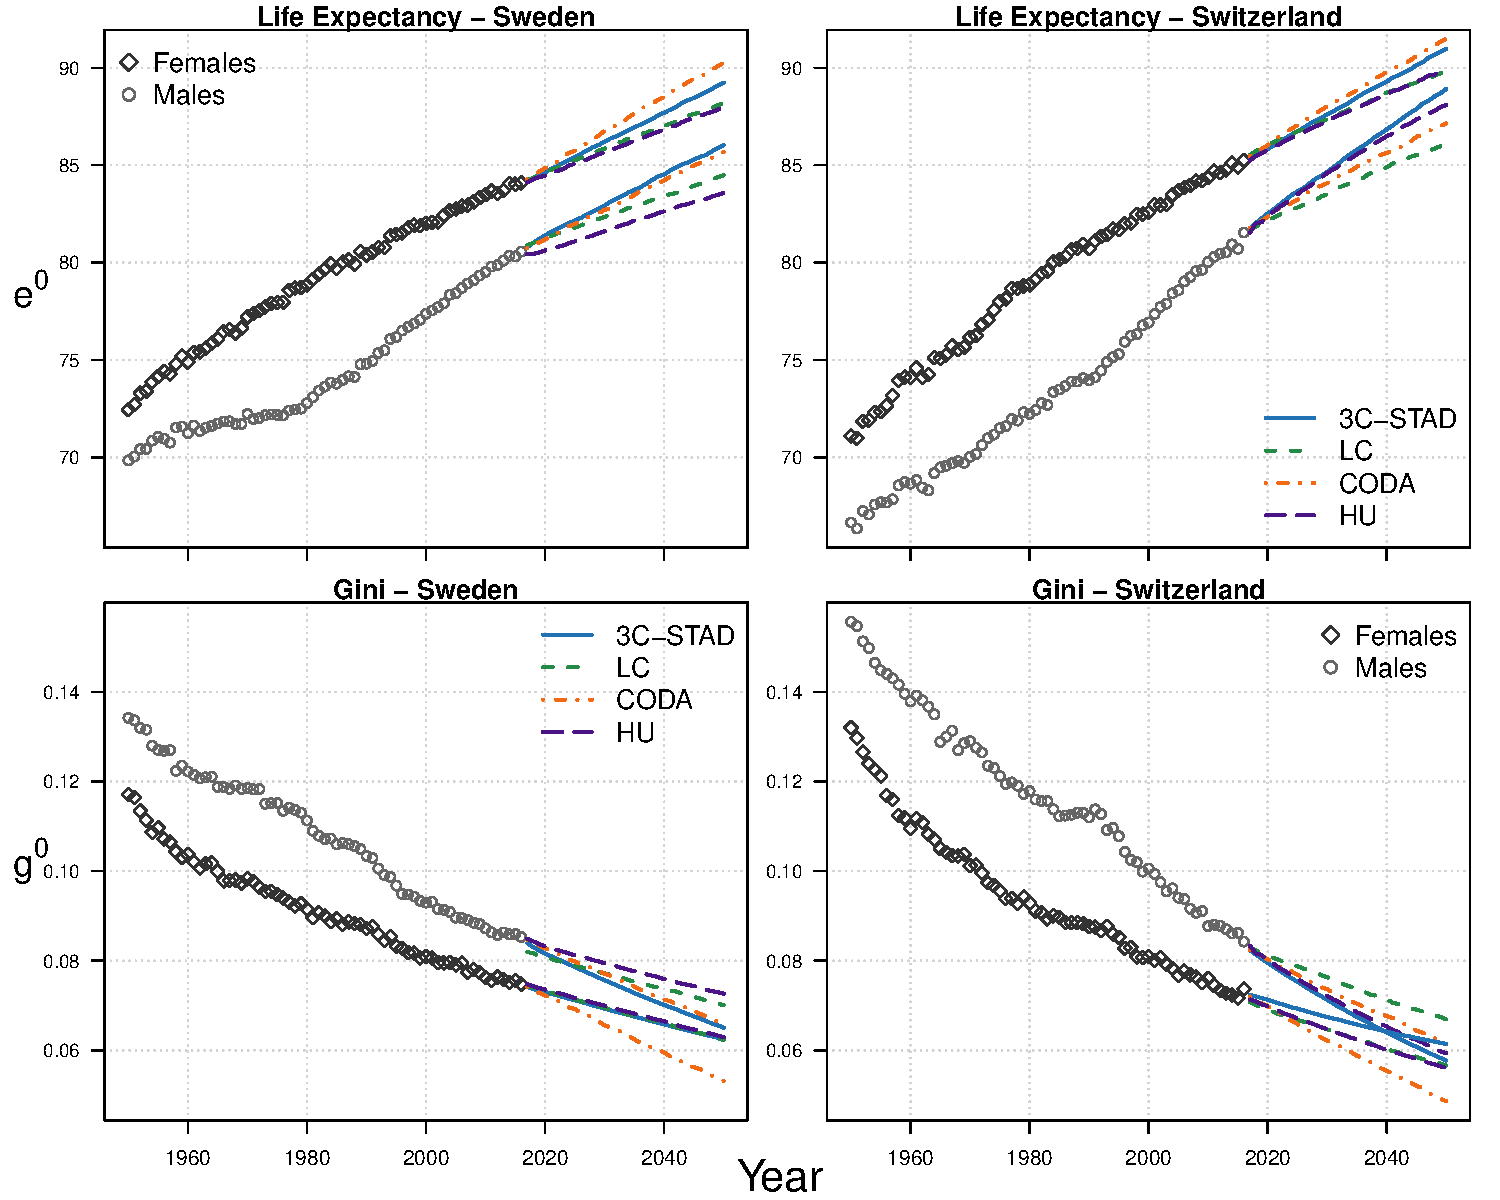
\includegraphics[scale=0.64]{./Figures/F4.pdf}
		\caption{Observed and forecast life expectancy at birth ($e^{0}$, top panels) and Gini coefficient ($g^{0}$, bottom panels) females and males in Sweden and Switzerland, 1950-2050. \\\footnotesize{\textit{Source}: as for Figure \ref{Fig:Intro}.} \label{Fig:e0g0fore}}		
	\end{center}
\end{figure}

\begin{figure}[h!]
	\begin{center}
		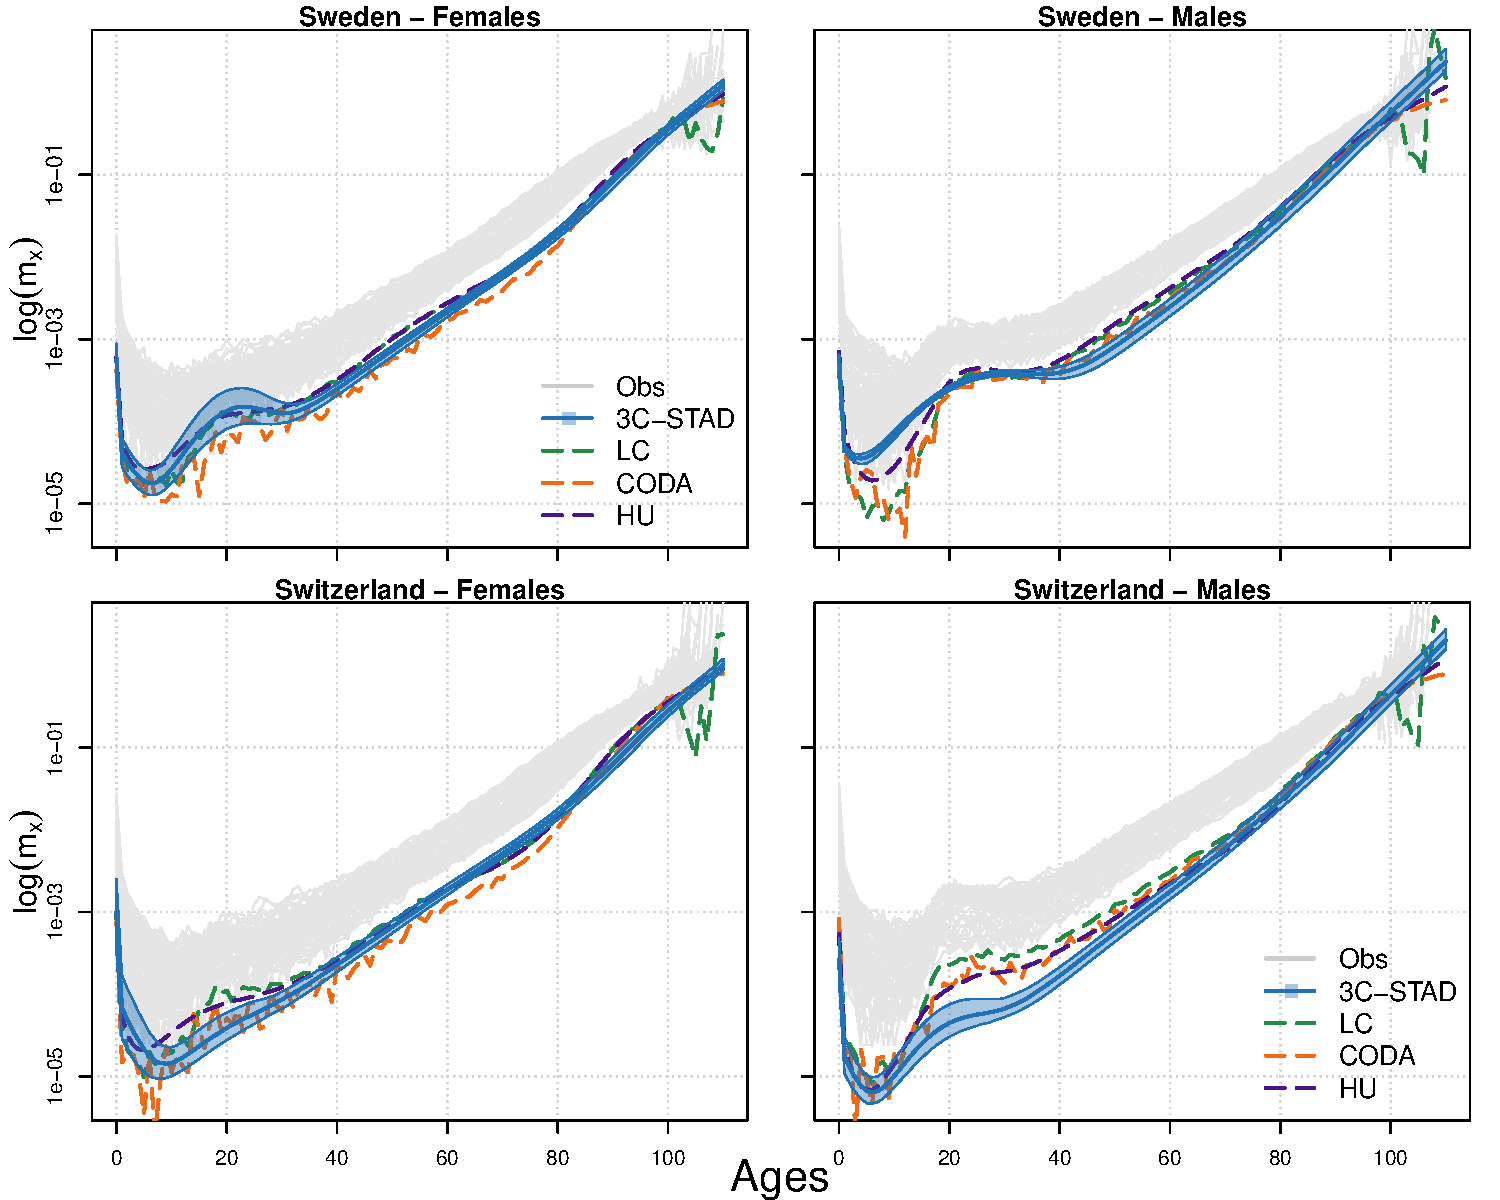
\includegraphics[scale=0.64]{./Figures/F5.pdf}
		\caption{Observed age-specific mortality rates in 1950--2016 (grey lines) and forecast rates of four models in 2050 for females and males in Sweden and Switzerland. Shaded areas correspond to 80\% PI for the 3C-STAD model. \\\footnotesize{\textit{Source}: as for Figure \ref{Fig:Intro}.} \label{Fig:LMXfore}}		
	\end{center}
\end{figure}

\begin{figure}[t]
	\begin{center}
		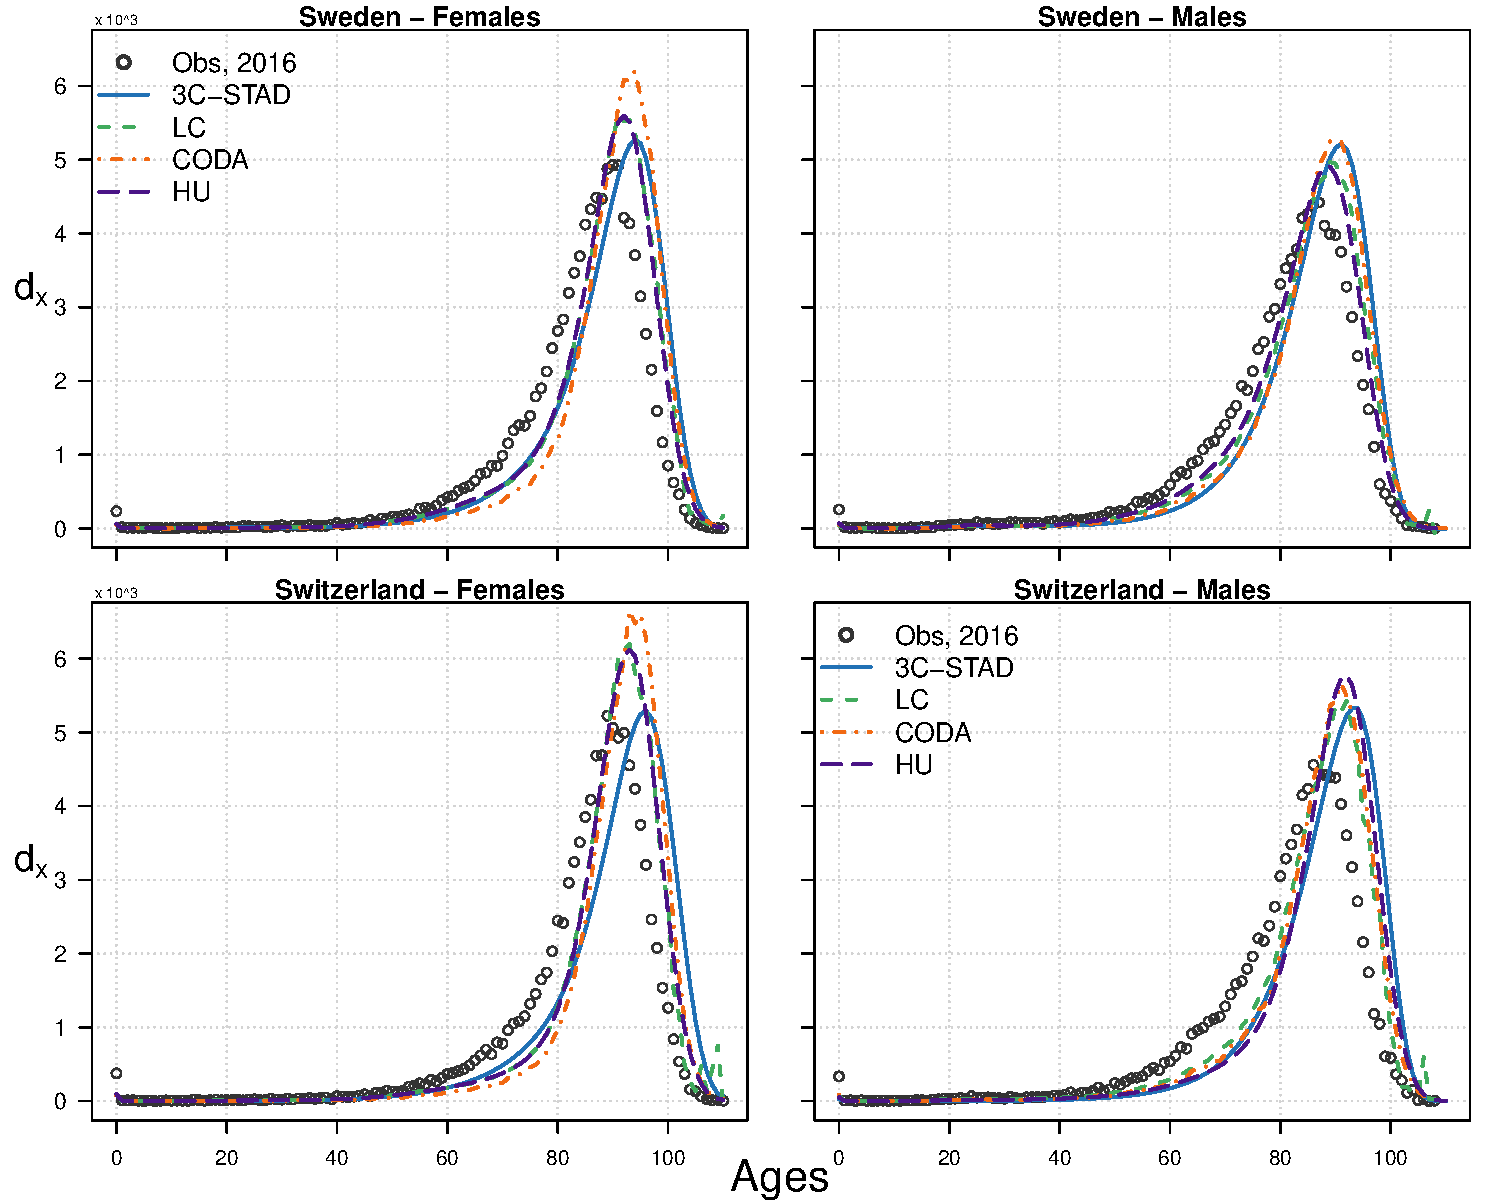
\includegraphics[scale=0.64]{./Figures/F6.pdf}
		\caption{Observed age-at-death distribution in 2016 (grey points) and forecasts of four models in 2050 for females and males in Sweden and Switzerland. \\\footnotesize{\textit{Source}: as for Figure \ref{Fig:Intro}.} \label{Fig:DXfore}}		
	\end{center}
\end{figure}

%%%%%%%%%%%%%%%%%%%%%%%%%%%%%%%%%%----------------------------%%%%%%%%%%%%%%%%%%%%%%%%%%%%%%%%%%----------------------------

\section{Discussion}\label{Sec:Discussion}

Age-at-death distributions have generally been neglected for modelling and forecasting mortality, despite providing insightful information on mortality age-patterns and trends over time. In this chapter, we introduced a novel stochastic methodology to forecast mortality that is based on changes in age-at-death distributions. Our proposed Three-Component Segmented Transformation Age-at-death Distributions (3C-STAD) model captures and forecasts mortality developments over age and time by: (i) decomposing mortality into three independent components, namely Childhood, Early-adulthood and Senescence, and (ii) modelling and forecasting changes in each component-specific age-at-death distributions. 

The decomposition of the mortality age-pattern into multiple components has a long history in demographic analysis. In \citeyear{thiele1871mathematical}, \citeauthor{thiele1871mathematical} pioneered this decomposition by expressing the force of mortality as the sum of three independent components that operate principally, or almost exclusively, upon childhood, middle and old ages, respectively. Shortly afterwards, \cite{lexis1878duree} theorized a similar three-component decomposition, but he shifted the attention from the force of mortality to the age-at-death distribution. His ideas were followed upon and further elaborated by \cite{pearson1897chances}, who divided the death density into five components, each one with its own distribution with different masses and degree of skewness. Finally, more recently, different parametric approaches have been proposed to decompose human mortality patterns \citep{siler1979competing,heligman1980age,kostaki1992nine,de2016new,mazzuco2018mortality}.

For our purposes, we performed a non-parametric decomposition using the Sum of Smooth Exponentials (SSE) model \citep{camarda2016sums}. We favour this over other parametric approaches because it allows us to achieve a good fit to the observed data without imposing a rigid parametric structure, hence adapting the decomposition to a large and diverse range of mortality developments. Moreover, via the SSE model, we obtain smooth components with specific shape constraints, and a two-dimensional age-time perspective is incorporated into the mortality decomposition. Component-specific age-at-death distributions derived by the SSE model are then isolated to model and forecast their changes. To do so, we employ modified versions of the relational model proposed by \cite{basellini2019stad}, originally designed for forecasting only adult distributions of deaths.

We have applied the 3C-STAD model to the female and male populations of Sweden and Switzerland using data retrieved from the \cite{HMD}. First, we assessed the point and interval forecast accuracy of the model by performing three out-of sample validation exercises. We have then forecast mortality for each population until 2050. In both cases, we compared the 3C-STAD projections with those of three well-known and employed methodologies: the \citeauthor{lee1992modeling} (LC, \citeyear{lee1992modeling}), the CODA \citep{oeppen2008coherent} and the \citeauthor{hyndman2007robust} (HU, \citeyear{hyndman2007robust}) models. We compare forecasts of summary measures, such as life expectancy as birth ($e^{0}$) and lifespan inequality (as measured by the Gini coefficient, $g^{0}$), as well as age-specific functions, such as death rates or age-at-death distributions.

The results of the out-of sample validation exercises show that the 3C-STAD produces accurate mortality forecasts, both in terms of point forecasts and prediction intervals (PI). In particular, the 3C-STAD was the most accurate model for point forecasts with respect to other models. Additionally, the 3C-STAD PI outperformed the other models for one indicator out of {\color{red}three} (see Table \ref{Table:Validation}). 

Concerning interval forecasts, CODA was found relatively more accurate, a result that might be related to the fact that ``the PI are wider with a CODA method than with an LC method" \cite[][p.~546]{bergeron2017coherent}. {\color{red}However, when we considered point and interval forecasts simultaneously using a proper scoring rule, the wide PI of the CODA were penalized to make it the worst performer across the four models.} Within 3C-STAD framework, a possibility to improve estimation of PI would be to include the uncertainty related to the SSE decomposition. However, preliminary analyses showed that this approach raises computational burden without a significant widening of the forecast variability. It is likely that the reason is due to our usage of the SSE model. In the decomposition procedure, we aim to follow mortality data as close as possible, consequently the SSE model presents extremely small uncertainty. Nonetheless, we envisage alternative procedures to further improve estimation of the interval accuracy of the 3C-STAD model.

Mortality forecasts until 2050 for the four populations highlighted additional differences between models. The 3C-STAD and CODA forecasts of $e^{0}$ are generally more optimistic than those of the LC and HU models. Forecasting age-at-death distributions instead of mortality rates here translates into more optimistic forecast of life expectancy, a preliminary finding already observed elsewhere \citep{bergeron2017what}. This could be an advantage, given that the LC forecasts have often under-predicted future gains in life expectancy \citep{lee2001evaluating}. Significant differences further emerge from an age-specific analysis of the different projections. On one side, the 3C-STAD forecast rates are inherently smooth, which is a desirable property especially for long-term projections \citep{li2013extending}. On the other side, the 3C-STAD forecast age-at-death distributions are characterized by greater shifting and smaller compression than those of other models. These projections seem more plausible, given that the shifting mortality dynamic has replaced the compression one in high-longevity countries in the most recent decades \citep{canudas2008modal,bergeron2015decomposing,janssen2019timing}. 
 
In general, we regard three characteristics as desirable for any forecasting methodology. First, the model should be able to capture and forecast mortality trends that can move in different directions across ages. Second, the relevant dynamics of mortality changes observed during the last century, i.e.~shift and compression, should be appropriately accounted for. Third, the forecast age-profile of mortality rates should be smooth, without implausible jaggedness where rates of adjacent age groups have very different and volatile values. Despite being one of the most employed forecasting methodology by public and private companies, the seminal LC model does not satisfy any of these properties. The single time index regulates the direction of change for mortality rates at all ages, i.e.~mortality improvements occur in the same direction at all ages. Furthermore, the model cannot account for the two mortality dynamics, and forecasts age-pattern are very volatile and jagged (see Figures \ref{Fig:LMXfore} and \ref{Fig:DXfore}).
 
Conversely, the 3C-STAD model meets all these three requirements. On one hand, the mortality decomposition allows us to capture and forecast mortality improvements across ages without rigid assumptions. Smoothness in the fitted and forecast age-profiles is a by-product of the non-parametric decomposition that we have employed. On the other hand, the 3C-STAD parameters capture and disentangle the shifting and compression mortality dynamics. The recently proposed model of \cite{bardoutsos2018projecting} is another example of projection methodology that satisfies these features.

Obviously, the 3C-STAD is not free of shortcomings, and neither we claim here that it outperforms all other forecasting methodologies. In addition to the width of the PI mentioned before, the computational time needed to produce mortality forecasts could be improved. The estimation of the two-dimensional SSE model in fact generally requires around thirty minutes, and speeding this step up will be required to shorten computational times. Future mortality values are obtained by forecasting eight time-series. Although this feature might pose issues in other situations, all of these series have clear demographic meanings and rather intelligible trends. Combination of univariate and multivariate time-series approaches has thus provided a reliable tool for overcoming this seemingly critical drawback of the 3C-STAD model. Different approaches in extrapolating the eight time-series will be pursuit, also for assessing consequences of specific future demographic scenarios. Moreover, in line with recent literature \citep{li2005coherent,hyndman2013coherent,janssen2013smoking,bergeron2017coherent}, future research will be directed towards the inclusion of coherence as an additional factor to improve forecasts for a group of (sub)populations.    

To conclude, we have shown that the proposed 3C-STAD model offers great prospects for modelling and forecasting human mortality. In light of the generally pessimistic forecasts of the widely employed LC model \citep{li2013extending,seligman2016convergence}, forecasting methodologies, such as the 3C-STAD, should be explored by pension and insurance providers to better assess their solvency needs, and by statistical bureaus to produce alternative population projections. 

\bibliographystyle{apalike}
\small
\bibliography{Biblio}

	
\end{document}	
